% Guia explicativo do projeto --- tudo o que foi feito, do formato aos resultados, sem o formato de artigo
% Compilar: latexmk -pdf guia.tex   (ou, na raiz do repositório: make paper)
\documentclass[11pt,a4paper]{article}

\usepackage[T1]{fontenc}
\usepackage[utf8]{inputenc}
\usepackage[brazilian]{babel}
\usepackage{lmodern}
\usepackage[margin=2.4cm]{geometry}
\usepackage{amsmath,amssymb}
\usepackage{booktabs}
\usepackage{tabularx}
\usepackage{array}
\usepackage{listings}
\usepackage{xcolor}
\usepackage{tikz}
\usetikzlibrary{arrows.meta,positioning,calc}
\usepackage{pgfplots}
\usepgfplotslibrary{groupplots}
\pgfplotsset{compat=1.18}
\usepackage{enumitem}
\usepackage{float}
\usepackage[hidelinks]{hyperref}

\lstset{
  basicstyle=\ttfamily\small,
  columns=fullflexible,
  keepspaces=true,
  frame=single,
  framesep=4pt,
  rulecolor=\color{black!30},
  showstringspaces=false,
  breaklines=true,
  extendedchars=true,
  literate=
    {á}{{\'a}}1 {à}{{\`a}}1 {ã}{{\~a}}1 {â}{{\^a}}1
    {é}{{\'e}}1 {ê}{{\^e}}1 {í}{{\'i}}1 {ó}{{\'o}}1
    {õ}{{\~o}}1 {ô}{{\^o}}1 {ú}{{\'u}}1 {ç}{{\c{c}}}1
    {Á}{{\'A}}1 {É}{{\'E}}1 {Ç}{{\c{C}}}1 {º}{{\textordmasculine}}1
    {—}{{---}}1 {–}{{--}}1 {−}{{-}}1 {≥}{{$\geq$}}1 {≤}{{$\leq$}}1
    {×}{{$\times$}}1 {→}{{$\rightarrow$}}1
}
\renewcommand{\lstlistingname}{Código}

\newcommand{\code}[1]{\texttt{#1}}
\newcommand{\res}{../../results}
% Gerado por: python3 -m sim.paper_numbers (não editar à mão)
\newcommand{\ERRTABLE}{T8 & \boldmath$1{,}6\times10^{0}$ & $6{,}8\times10^{-2}$ & \boldmath$2{,}1\times10^{-1}$ & $7{,}7\times10^{-2}$ & $1{,}1\times10^{-1}$ & $1{,}4\times10^{-1}$ & $5{,}7\times10^{-2}$ & \boldmath$5{,}4\times10^{-1}$ & $1{,}4\times10^{-1}$\\
FP8 & $1{,}6\times10^{0}$ & $7{,}7\times10^{-2}$ & $\infty$ & $9{,}0\times10^{-2}$ & $5{,}4\times10^{-2}$ & $6{,}4\times10^{-2}$ & $4{,}4\times10^{-2}$ & $\infty$ & $7{,}2\times10^{-2}$\\
FP8w & $1{,}7\times10^{0}$ & \boldmath$4{,}4\times10^{-2}$ & $\infty$ & \boldmath$4{,}1\times10^{-2}$ & \boldmath$3{,}8\times10^{-2}$ & \boldmath$5{,}1\times10^{-2}$ & \boldmath$3{,}6\times10^{-2}$ & $\infty$ & \boldmath$6{,}4\times10^{-2}$\\
\midrule
T16 & \boldmath$6{,}9\times10^{-3}$ & \boldmath$2{,}7\times10^{-4}$ & $8{,}4\times10^{-4}$ & \boldmath$2{,}5\times10^{-4}$ & \boldmath$2{,}6\times10^{-4}$ & $5{,}4\times10^{-4}$ & \boldmath$2{,}3\times10^{-4}$ & \boldmath$2{,}0\times10^{-3}$ & $5{,}8\times10^{-4}$\\
FP16 & $9{,}1\times10^{-3}$ & $4{,}7\times10^{-4}$ & $3{,}8\times10^{-4}$ & $6{,}7\times10^{-4}$ & $3{,}9\times10^{-4}$ & $3{,}5\times10^{-4}$ & $2{,}9\times10^{-4}$ & $\infty$ & $3{,}8\times10^{-4}$\\
FP16w & $9{,}0\times10^{-3}$ & $3{,}2\times10^{-4}$ & \boldmath$2{,}4\times10^{-4}$ & $3{,}2\times10^{-4}$ & $3{,}0\times10^{-4}$ & \boldmath$3{,}1\times10^{-4}$ & $2{,}4\times10^{-4}$ & $\infty$ & \boldmath$3{,}1\times10^{-4}$\\
\midrule
T32 & \boldmath$9{,}9\times10^{-8}$ & \boldmath$4{,}2\times10^{-9}$ & \boldmath$1{,}4\times10^{-8}$ & \boldmath$3{,}4\times10^{-9}$ & \boldmath$3{,}7\times10^{-9}$ & \boldmath$8{,}3\times10^{-9}$ & \boldmath$3{,}8\times10^{-9}$ & \boldmath$3{,}3\times10^{-8}$ & \boldmath$8{,}6\times10^{-9}$\\
FP32 & $1{,}2\times10^{-6}$ & $6{,}9\times10^{-8}$ & $5{,}2\times10^{-8}$ & $1{,}0\times10^{-7}$ & $4{,}6\times10^{-8}$ & $5{,}2\times10^{-8}$ & $3{,}7\times10^{-8}$ & $6{,}2\times10^{-8}$ & $4{,}8\times10^{-8}$\\
FP32w & $9{,}3\times10^{-7}$ & $4{,}3\times10^{-8}$ & $3{,}1\times10^{-8}$ & $3{,}8\times10^{-8}$ & $3{,}5\times10^{-8}$ & $3{,}8\times10^{-8}$ & $3{,}0\times10^{-8}$ & $4{,}0\times10^{-8}$ & $3{,}8\times10^{-8}$\\}
\newcommand{\ERRTABLESYN}{T8 & \boldmath$1{,}6\times10^{0}$ & $6{,}8\times10^{-2}$ & \boldmath$2{,}1\times10^{-1}$ & $7{,}7\times10^{-2}$\\
FP8 & $1{,}6\times10^{0}$ & $7{,}7\times10^{-2}$ & $\infty$ & $9{,}0\times10^{-2}$\\
FP8w & $1{,}7\times10^{0}$ & \boldmath$4{,}4\times10^{-2}$ & $\infty$ & \boldmath$4{,}1\times10^{-2}$\\
\midrule
T16 & \boldmath$6{,}9\times10^{-3}$ & \boldmath$2{,}7\times10^{-4}$ & $8{,}4\times10^{-4}$ & \boldmath$2{,}5\times10^{-4}$\\
FP16 & $9{,}1\times10^{-3}$ & $4{,}7\times10^{-4}$ & $3{,}8\times10^{-4}$ & $6{,}7\times10^{-4}$\\
FP16w & $9{,}0\times10^{-3}$ & $3{,}2\times10^{-4}$ & \boldmath$2{,}4\times10^{-4}$ & $3{,}2\times10^{-4}$\\
\midrule
T32 & \boldmath$9{,}9\times10^{-8}$ & \boldmath$4{,}2\times10^{-9}$ & \boldmath$1{,}4\times10^{-8}$ & \boldmath$3{,}4\times10^{-9}$\\
FP32 & $1{,}2\times10^{-6}$ & $6{,}9\times10^{-8}$ & $5{,}2\times10^{-8}$ & $1{,}0\times10^{-7}$\\
FP32w & $9{,}3\times10^{-7}$ & $4{,}3\times10^{-8}$ & $3{,}1\times10^{-8}$ & $3{,}8\times10^{-8}$\\}
\newcommand{\ERRTABLEREAL}{T8 & $1{,}1\times10^{-1}$ & $1{,}4\times10^{-1}$ & $5{,}7\times10^{-2}$ & \boldmath$5{,}4\times10^{-1}$ & $1{,}4\times10^{-1}$\\
FP8 & $5{,}4\times10^{-2}$ & $6{,}4\times10^{-2}$ & $4{,}4\times10^{-2}$ & $\infty$ & $7{,}2\times10^{-2}$\\
FP8w & \boldmath$3{,}8\times10^{-2}$ & \boldmath$5{,}1\times10^{-2}$ & \boldmath$3{,}6\times10^{-2}$ & $\infty$ & \boldmath$6{,}4\times10^{-2}$\\
\midrule
T16 & \boldmath$2{,}6\times10^{-4}$ & $5{,}4\times10^{-4}$ & \boldmath$2{,}3\times10^{-4}$ & \boldmath$2{,}0\times10^{-3}$ & $5{,}8\times10^{-4}$\\
FP16 & $3{,}9\times10^{-4}$ & $3{,}5\times10^{-4}$ & $2{,}9\times10^{-4}$ & $\infty$ & $3{,}8\times10^{-4}$\\
FP16w & $3{,}0\times10^{-4}$ & \boldmath$3{,}1\times10^{-4}$ & $2{,}4\times10^{-4}$ & $\infty$ & \boldmath$3{,}1\times10^{-4}$\\
\midrule
T32 & \boldmath$3{,}7\times10^{-9}$ & \boldmath$8{,}3\times10^{-9}$ & \boldmath$3{,}8\times10^{-9}$ & \boldmath$3{,}3\times10^{-8}$ & \boldmath$8{,}6\times10^{-9}$\\
FP32 & $4{,}6\times10^{-8}$ & $5{,}2\times10^{-8}$ & $3{,}7\times10^{-8}$ & $6{,}2\times10^{-8}$ & $4{,}8\times10^{-8}$\\
FP32w & $3{,}5\times10^{-8}$ & $3{,}8\times10^{-8}$ & $3{,}0\times10^{-8}$ & $4{,}0\times10^{-8}$ & $3{,}8\times10^{-8}$\\}
\newcommand{\RATA}{1{,}2}
\newcommand{\RATB}{11}
\newcommand{\WIDET}{$8{,}4\times10^{-4}$}
\newcommand{\WIDEF}{$2{,}4\times10^{-4}$}
\newcommand{\BUST}{$5{,}4\times10^{-4}$}
\newcommand{\BUSF}{$3{,}1\times10^{-4}$}
\newcommand{\WIDETEIGHT}{$2{,}1\times10^{-1}$}
\newcommand{\BCSTEIGHT}{$5{,}4\times10^{-1}$}
\newcommand{\BCSTSIXTEEN}{$2{,}0\times10^{-3}$}
\newcommand{\FPEIGHTBAD}{217}
\newcommand{\NFBUS}{94}
\newcommand{\NFWEST}{51}
\newcommand{\NFBCS}{153}
\newcommand{\NFWESTH}{5}
\newcommand{\NFBCSH}{149}
\newcommand{\MEMTE}{$1{,}4\times10^{-1}$}
\newcommand{\MEMTEBAD}{267}
\newcommand{\MEMFE}{$6{,}4\times10^{-2}$}
\newcommand{\MEMFEBAD}{1\,054}
\newcommand{\MEMTS}{$5{,}8\times10^{-4}$}
\newcommand{\MEMTSBAD}{3}
\newcommand{\MEMFS}{$3{,}1\times10^{-4}$}
\newcommand{\MEMFSBAD}{2}
\newcommand{\MEMTT}{$8{,}6\times10^{-9}$}
\newcommand{\MEMTTBAD}{0}
\newcommand{\MEMFT}{$3{,}8\times10^{-8}$}
\newcommand{\MEMFTBAD}{0}
\newcommand{\MEMROWS}{17\,758}
\newcommand{\MATTABLE}{poisson & 256$\times$256 & 1\,216 & 4{,}8 & $2^{0}$ -- $2^{2}$\\
gauss & 256$\times$256 & 2\,560 & 10{,}0 & $2^{-13}$ -- $2^{2}$\\
wide & 256$\times$256 & 2\,560 & 10{,}0 & $2^{-10}$ -- $2^{10}$\\
mlp & 256$\times$512 & 13\,056 & 51{,}0 & $2^{-15}$ -- $2^{0}$\\
\midrule
nos4 & 100$\times$100 & 594 & 5{,}9 & $2^{-6}$ -- $2^{-1}$\\
bus494 & 494$\times$494 & 1\,666 & 3{,}4 & $2^{-3}$ -- $2^{14}$\\
west0479 & 479$\times$479 & 1\,910 & 4{,}0 & $2^{-21}$ -- $2^{18}$\\
bcsstk05 & 153$\times$153 & 2\,423 & 15{,}8 & $2^{-31}$ -- $2^{22}$\\
memplus & 17758$\times$17758 & 126\,150 & 7{,}1 & $2^{-86}$ -- $2^{0}$\\}
\newcommand{\INSTRTABLE}{poisson & 4{,}8 & 6\,146 & 6\,146 & 6\,658 & 0{,}0\% & 7{,}7\%\\
gauss & 10{,}0 & 8\,962 & 9\,218 & 9\,986 & 2{,}8\% & 10{,}3\%\\
mlp & 51{,}0 & 23\,042 & 24\,578 & 26\,626 & 6{,}2\% & 13{,}5\%\\
\midrule
nos4 & 5{,}9 & 2\,402 & 2\,402 & 2\,602 & 0{,}0\% & 7{,}7\%\\
bus494 & 3{,}4 & 11\,902 & 11\,906 & 12\,898 & 0{,}0\% & 7{,}7\%\\
west0479 & 4{,}0 & 11\,949 & 11\,990 & 12\,989 & 0{,}3\% & 8{,}0\%\\
bcsstk05 & 15{,}8 & 6\,061 & 6\,278 & 6\,801 & 3{,}5\% & 10{,}9\%\\
memplus & 7{,}1 & 503\,161 & 510\,158 & 552\,671 & 1{,}4\% & 9{,}0\%\\}
\newcommand{\SAVEWLO}{7{,}7}
\newcommand{\SAVEWHI}{14{,}3}
\newcommand{\SAVEPHI}{7{,}1}
\newcommand{\FLAGPCT}{90}
\newcommand{\FLAGWHERE}{\emph{wide}, FP32}
\newcommand{\HWDECA}{46}
\newcommand{\HWDECB}{89}
\newcommand{\HWDECC}{164}
\newcommand{\HWENCA}{70}
\newcommand{\HWENCB}{118}
\newcommand{\HWENCC}{216}
\newcommand{\HWALUA}{327}
\newcommand{\HWALUB}{912}
\newcommand{\HWALUC}{2\,838}
\newcommand{\HWNCA}{32}
\newcommand{\HWNCB}{67}
\newcommand{\HWNCC}{155}
\newcommand{\HWWMA}{220}
\newcommand{\HWWMB}{686}
\newcommand{\HWWMC}{2\,384}
\newcommand{\HWDOTA}{6\,740}
\newcommand{\HWDOTB}{7\,525}
\newcommand{\HWDOTC}{9\,451}
\newcommand{\HWHDR}{41}

\newcommand{\cdf}[3][]{\addplot+[no markers, #1] table[x=err, y=frac] {\res/cdf_#2_#3.dat};}
\newcommand{\matplot}[2][]{%
  \nextgroupplot[title={#2}, #1]
  \cdf[blue!75!black]{#2}{T8}    \cdf[blue!75!black, dashed]{#2}{FP8w}
  \cdf[red!75!black]{#2}{T16}    \cdf[red!75!black, dashed]{#2}{FP16w}
  \cdf[green!45!black]{#2}{T32}  \cdf[green!45!black, dashed]{#2}{FP32w}}
% campo de bits colorido
\newcommand{\bS}[1]{\colorbox{gray!25}{\texttt{#1}}}
\newcommand{\bD}[1]{\colorbox{blue!18}{\texttt{#1}}}
\newcommand{\bR}[1]{\colorbox{blue!8}{\texttt{#1}}}
\newcommand{\bC}[1]{\colorbox{orange!25}{\texttt{#1}}}
\newcommand{\bF}[1]{\colorbox{green!18}{\texttt{#1}}}
\setlength{\fboxsep}{1.5pt}

\title{\textbf{Guia do Projeto Zvtakum}\\[4pt]
\large Tudo o que foi feito, explicado passo a passo\\[2pt]
\normalsize Projeto Integrador AOC 2026/02 --- Formato Takum na Extensão Vetorial RISC-V}
\author{Heloisa Silva Rosa \and Samantha Kelly de Souza Sena \and Vitor Hugo Lacerda Lana\\[4pt]
  \small Arquitetura e Organização de Computadores --- DELT/UFMG}
\date{Novembro de 2026}

\begin{document}
\maketitle

\noindent Este documento explica o projeto inteiro em linguagem direta: o que o enunciado pedia, o que
construímos, como cada parte funciona, como sabemos que está certa e o que os resultados significam.
Ele não é o artigo. O artigo (\code{docs/artigo/}) é curto e formal; aqui há exemplos feitos à mão, os
porquês das decisões e as perguntas que alguém de fora faria. Todos os números vêm dos arquivos em
\code{results/} e podem ser regenerados com os comandos da Seção~\ref{sec:repro}.

\tableofcontents

%======================================================================
\section{O projeto em uma página}

\paragraph{O problema.} Os processadores vetoriais vêm acumulando formatos de ponto flutuante pequenos
(16 e 8 bits) para inteligência artificial. Todos derivam do padrão IEEE~754, e cada um traz sua largura
de expoente, seus casos especiais e suas conversões. Isso custa instruções, lógica de exceção e
registradores de controle.

\paragraph{A proposta estudada.} O \emph{takum} é um formato numérico de Laslo Hunhold (2024) em que a
mesma regra vale para qualquer número de bits. O enunciado pede para (1) implementar o takum em hardware,
(2) propor instruções vetoriais RISC-V que o usem, a extensão \emph{Zvtakum}, e (3) comparar com o
IEEE~754 em um problema real de álgebra linear.

\paragraph{O que entregamos.}
\begin{center}
\begin{tabularx}{\linewidth}{lX}
\toprule
Fase do enunciado & O que existe no repositório \\
\midrule
1. Decodificação e aritmética & Decodificador, codificador e ALU (soma, subtração, multiplicação) em
   Verilog, para 8, 16 e 32 bits \\
2. Extensão do conjunto de instruções & As cinco instruções da Zvtakum em hardware e uma codificação
   binária para elas; um simulador que executa programas RISC-V com essas instruções \\
3. Avaliação experimental & Produto de matriz esparsa por vetor em takum e em IEEE~754, com nove
   matrizes (quatro geradas e cinco reais, de repositório público, uma delas com quase 18 mil linhas); erro contra precisão quádrupla;
   contagem de instruções; análise dos registradores de controle \\
Documentos & Artigo em inglês e em português, slides, este guia \\
\bottomrule
\end{tabularx}
\end{center}

\paragraph{As conclusões, em quatro frases.}
\begin{enumerate}[nosep]
  \item Em 32 bits o takum erra menos que o IEEE nas nove matrizes (de \RATA{} a \RATB{} vezes menos).
  \item Em 16 bits ele ganha quando os números estão perto de 1, perde quando estão moderadamente
        espalhados e continua respondendo quando o IEEE estoura (em uma matriz real, o binary16 devolveu
        infinito ou NaN em \NFBCSH{} de 153 resultados).
  \item Em 8 bits o takum é \emph{menos} preciso que o IEEE quando os dados cabem na faixa (até 3 vezes),
        mas nunca estoura: o IEEE de 8 bits devolveu infinito ou NaN em quatro das nove matrizes, em uma
        delas em todas as linhas.
  \item O conjunto de instruções fica mais simples: nenhum registrador de controle de ponto flutuante,
        comparações e conversões viram operações inteiras, e o produto escalar em uma instrução economiza
        de 8 a 14\% das instruções executadas.
\end{enumerate}

%======================================================================
\section{Mapa do repositório}

\begin{center}
\begin{tabularx}{\linewidth}{lX}
\toprule
Pasta ou arquivo & Conteúdo \\
\midrule
\code{rtl/} & O hardware, em Verilog: \code{takum\_hdr\_dec} (cabeçalho), \code{takum\_decoder},
  \code{takum\_encoder}, \code{takum\_alu}, \code{takum\_wmul} (produto alargado), \code{takum\_ncvt}
  (redução de largura), \code{takum\_dot} (produto escalar), \code{takum\_vec\_alu} (unidade vetorial) \\
\code{tb/} & Os testes do hardware e o \emph{oráculo} \code{takum\_oracle.py}, que calcula a resposta
  certa com aritmética exata \\
\code{sim/} & O simulador RISC-V em Python: formatos numéricos, montador, a máquina, os programas de teste
  e o experimento \\
\code{data/matrixmarket/} & As cinco matrizes reais, baixadas do repositório Matrix Market (NIST), com
  um \code{LEIAME.md} dizendo de onde veio cada uma \\
\code{results/} & Os dados produzidos pelo experimento (CSV) \\
\code{docs/} & Revisão bibliográfica, relatórios, artigo, slides e este guia \\
\code{Makefile} & Um comando para cada coisa: \code{make test}, \code{make bench}, \code{make simdemo}\ldots \\
\bottomrule
\end{tabularx}
\end{center}

%======================================================================
\section{O formato takum na prática}

\subsection{Os campos}

Uma palavra takum de $n$ bits é lida da esquerda para a direita em cinco campos:

\begin{center}
\bS{S}\,\bD{D}\,\bR{R R R}\,\bC{C \ldots\ C}\,\bF{F \ldots\ F}
\qquad
\begin{tabular}{@{}ll@{}}
\bS{S} sinal (1 bit) & \bD{D} direção (1 bit)\\
\bR{R} regime (3 bits) & \bC{C} característica ($r$ bits, de 0 a 7)\\
\bF{F} fração (o que sobrar: $n-5-r$ bits) &
\end{tabular}
\end{center}

O regime diz quantos bits a característica ocupa; a característica dá o expoente; a fração dá os
dígitos. Para um número positivo:
\[
r = \begin{cases} R & \text{se } D=1\\ 7-R & \text{se } D=0 \end{cases}
\qquad
c = \begin{cases} 2^r - 1 + C & \text{se } D=1\\ -2^{r+1} + 1 + C & \text{se } D=0 \end{cases}
\qquad
x = (1 + f)\cdot 2^{c},
\]
em que $f$ é a fração lida como um número entre 0 e 1. O bit $D$ separa os números maiores ou iguais a 1
($D=1$, expoente $c\ge0$) dos menores que 1 ($D=0$, $c<0$).

\subsection{Três exemplos feitos à mão}

\paragraph{O número 3 em 8 bits} é \code{0x4A}:
\bS{0}\,\bD{1}\,\bR{001}\,\bC{0}\,\bF{10}.
$D=1$ e $R=1$ dão $r=1$: a característica tem 1 bit, $C=0$, logo $c=2^1-1+0=1$. Sobram 2 bits de fração,
\code{10}, isto é, $f=0{,}5$. Então $x=(1+0{,}5)\cdot2^1=3$.

\paragraph{O número 12,75 em 16 bits} é \code{0x5130}:
\bS{0}\,\bD{1}\,\bR{010}\,\bC{00}\,\bF{100110000}.
$r=2$, $C=0$, logo $c=2^2-1=3$. A fração tem 9 bits e vale $304/512=0{,}59375$. Então
$x=1{,}59375\cdot 8=12{,}75$.

\paragraph{O número $-1{,}5$ em 8 bits} é \code{0xBC}. Números negativos são o complemento de dois da
palavra do número positivo: negando \code{0xBC} obtemos \code{0x44} $=$
\bS{0}\,\bD{1}\,\bR{000}\,\bF{100}, que tem $r=0$ (nenhum bit de característica), $c=0$ e
$f=0{,}5$, ou seja, $1{,}5$.

\subsection{Precisão afunilada}

Como a característica rouba bits da fração, a precisão depende do tamanho do número. É isso que
\emph{precisão afunilada} quer dizer.

\begin{center}
\begin{tabular}{lcccc}
\toprule
Faixa do valor (em módulo) & $r$ & Fração em T8 & em T16 & em T32\\
\midrule
de 0,5 a 2 & 0 & 3 bits & 11 & 27\\
de 2 a 8, ou de 0,125 a 0,5 & 1 & 2 & 10 & 26\\
de 8 a 128 & 2 & 1 & 9 & 25\\
de 128 a $32\,768$ ($2^{7}$ a $2^{15}$) & 3 & 0 & 8 & 24\\
\ldots & \ldots & & & \\
os maiores, até $2^{254}$ & 7 & 0 & 4 & 20\\
\bottomrule
\end{tabular}
\end{center}

Compare com o IEEE, que tem sempre a mesma fração: 3 bits no FP8 (E4M3), 10 no binary16, 23 no binary32.
Perto de 1 o takum tem \emph{mais} bits que o IEEE de mesma largura (11 contra 10; 27 contra 23); longe
de 1, menos. Guarde esta tabela: ela explica todos os resultados da Seção~\ref{sec:exp}.

Em troca, a faixa é enorme. O maior número de 8 bits no nosso FP8 é 240; o maior takum de 8 bits é
$2^{239}\approx 8{,}8\cdot10^{71}$. A partir de 12 bits a faixa do takum chega a $2^{\pm255}$ e não cresce
mais: aumentar a largura só acrescenta fração.

\subsection{Casos especiais e ordem}

\begin{itemize}[nosep]
  \item \code{00\ldots0} é o zero. Só existe um zero (o IEEE tem $+0$ e $-0$).
  \item \code{10\ldots0} é o NaR (\emph{Not a Real}), o resultado de uma operação sem resposta. Só existe
        um (o IEEE tem dois infinitos e milhões de NaN).
  \item Não há subnormais nem infinitos. Um resultado grande demais satura no maior número; um pequeno
        demais, no menor número positivo. Nunca vira zero nem NaR por arredondamento.
  \item Lidas como inteiros com sinal, as palavras ficam \textbf{na mesma ordem} dos valores que
        representam. Para comparar dois takums basta o comparador de inteiros.
\end{itemize}

A última propriedade tem uma consequência que usamos em todo o hardware: \textbf{somar 1 à palavra leva
ao próximo número representável}. Arredondar para cima é incrementar.

%======================================================================
\section{O hardware}

\subsection{Três blocos em sequência}

Toda operação segue o mesmo caminho: \emph{decodificar} os operandos, \emph{calcular} e \emph{codificar}
o resultado.

\begin{figure}[H]
\centering
\begin{tikzpicture}[
  blk/.style={draw, rounded corners=2pt, minimum height=9mm, align=center, font=\small},
  arr/.style={-{Latex[length=2mm]}}]
  \node[blk, minimum width=26mm] (da) at (0, 0.8) {decodificador};
  \node[blk, minimum width=26mm] (db) at (0,-0.8) {decodificador};
  \node[blk, minimum width=28mm, minimum height=25mm] (core) at (4.3,0) {núcleo\\ soma / subtração /\\ multiplicação};
  \node[blk, minimum width=28mm] (enc) at (8.6,0) {codificador\\ \scriptsize arredonda e satura};
  \node (a) at (-2.3, 0.8) {$a$}; \node (b) at (-2.3,-0.8) {$b$}; \node (y) at (10.9,0) {$y$};
  \draw[arr] (a) -- (da); \draw[arr] (b) -- (db);
  \draw[arr] (da.east) -- (core.west |- da.east);
  \draw[arr] (db.east) -- (core.west |- db.east);
  \draw[arr] (core) -- (enc); \draw[arr] (enc) -- (y);
\end{tikzpicture}
\caption{Caminho de dados da ALU (\code{rtl/takum\_alu.v}). Cada decodificador entrega sinal,
expoente e fração ao núcleo.}
\end{figure}

\paragraph{Decodificador.} Se a palavra é negativa, nega. Depois entrega os 12 bits de cima a um bloco
pequeno e fixo, o \code{takum\_hdr\_dec}, que devolve $r$ e o expoente $c$. Esse bloco é \emph{o mesmo}
para 8, 16 e 32 bits (custa \HWHDR{} LUTs), porque o cabeçalho S, D, R, C nunca passa de 12 bits. Por
fim, um deslocador alinha a fração. É a principal vantagem de hardware do takum: nos formatos IEEE cada
largura tem um expoente de tamanho diferente.

\paragraph{Núcleo.} Trabalha com sinal, expoente e \emph{significando} (o número $1{,}f$).
\begin{itemize}[nosep]
  \item \emph{Multiplicação:} soma os expoentes e multiplica os significandos. Se o produto passar de 2,
        ajusta o expoente em 1.
  \item \emph{Soma e subtração:} descobre qual operando é maior, desloca o menor para a direita até os
        expoentes coincidirem, soma ou subtrai e normaliza (procura o primeiro bit 1). A subtração é a
        soma com o sinal de $b$ trocado.
\end{itemize}
Os bits que não cabem no resultado são resumidos em três: \emph{guard}, \emph{round} e \emph{sticky}.
Eles bastam para decidir o arredondamento corretamente.

\paragraph{Codificador.} Monta a palavra de volta, arredonda e satura.

\subsection{Arredondar na palavra: um exemplo}

Quanto é $5\times3$ em takum de 8 bits? O resultado exato, 15, é $1{,}875\cdot2^3$. Com $c=3$ temos
$r=2$, e em 8 bits sobra \emph{um} bit de fração. A palavra exata, se tivéssemos bits de sobra, seria

\begin{center}
\bS{0}\,\bD{1}\,\bR{010}\,\bC{00}\,\bF{1}\;\;\Big|\;\;\bF{11}
\end{center}

A barra marca onde os 8 bits acabam. Os 8 bits de cima são \code{0x51}, que vale 12. Os bits descartados
(\code{11}) passam da metade, então arredondamos para cima: $\code{0x51}+1=\code{0x52}$. E \code{0x52} é
\bS{0}\,\bD{1}\,\bR{010}\,\bC{01}\,\bF{0}, que vale $2^4=16$.

O incremento mudou a característica de \code{00} para \code{01} sozinho, sem lógica extra. Os vizinhos
representáveis de 15 em T8 são 12 e 16, e 16 é o mais próximo: o resultado está certo. No código, o
arredondamento inteiro é este trecho do codificador:

\lstinputlisting[language=Verilog, firstline=57, lastline=62, firstnumber=57, numbers=left,
  numberstyle=\tiny\color{black!50}]{../../rtl/takum_encoder.v}

A regra é a do IEEE: para o mais próximo e, no empate exato, para a palavra par.

%======================================================================
\section{A extensão Zvtakum}

\subsection{As cinco instruções}

O RISC-V tem uma extensão vetorial, a RVV, com registradores \code{v0} a \code{v31} e instruções que
operam em vários elementos de uma vez. A Zvtakum é a nossa proposta de instruções takum dentro desse
modelo. Ela segue a tabela do enunciado:

\begin{center}
\begin{tabularx}{\linewidth}{llX}
\toprule
Instrução & Equivalente RVV & O que faz \\
\midrule
\code{vtadd.vv vd, vs2, vs1} & \code{vfadd.vv} & soma elemento a elemento \\
\code{vtsub.vv vd, vs2, vs1} & \code{vfsub.vv} & subtrai elemento a elemento ($vs2 - vs1$) \\
\code{vtmul.vv vd, vs2, vs1} & \code{vfmul.vv} & multiplica elemento a elemento \\
\code{vtdot.vv vd, vs2, vs1} & \code{vfwmul} + redução & produto escalar: soma em \code{vd[0]} os produtos
   $vs2_i\cdot vs1_i$, com o dobro da largura \\
\code{vncvt.t.t vd, vs2} & \code{vfncvt.f.f.w} & converte elementos de largura dupla para a largura
   simples (por exemplo, T16 para T8) \\
\bottomrule
\end{tabularx}
\end{center}

Três conceitos da RVV valem aqui sem mudança:
\begin{itemize}[nosep]
  \item \textbf{SEW} é a largura do elemento (8, 16 ou 32). Um registrador de 64 bits tem 8, 4 ou 2
        elementos.
  \item \textbf{\code{vl}} é quantos elementos a instrução deve processar. Os demais (a \emph{cauda})
        ficam como estavam.
  \item \textbf{Máscara:} com o sufixo \code{v0.t}, só são processados os elementos cujo bit em \code{v0}
        vale 1.
\end{itemize}

\subsection{Como ficam em binário}

Toda instrução RISC-V tem 32 bits. Usamos o mesmo desenho de campos das instruções vetoriais existentes:

\begin{center}
\small
\begin{tabular}{|c|c|c|c|c|c|c|}
\hline
\code{funct6} & \code{vm} & \code{vs2} & \code{vs1} & \code{funct3} & \code{vd} & \code{opcode}\\
6 bits & 1 & 5 & 5 & 3 & 5 & 7\\
\hline
\end{tabular}
\end{center}

Por exemplo, \code{vtadd.vv v3, v2, v1} é montada como \code{0x022091DB}:

\begin{center}
\small
\begin{tabular}{|c|c|c|c|c|c|c|}
\hline
\code{000000} & \code{1} & \code{00010} & \code{00001} & \code{001} & \code{00011} & \code{1011011}\\
soma & sem máscara & \code{v2} & \code{v1} & vetor--vetor & \code{v3} & \emph{custom-2}\\
\hline
\end{tabular}
\end{center}

A instrução IEEE equivalente, \code{vfadd.vv v3, v2, v1}, é \code{0x022091D7}. A única diferença está nos
7 bits finais: o \emph{opcode}. Foi uma escolha nossa. O RISC-V reserva alguns opcodes para extensões de
terceiros (os \emph{custom}), e usamos o \emph{custom-2}; mantendo todos os outros campos iguais aos da
instrução de ponto flutuante correspondente, o decodificador de um processador RVV serve quase sem
alteração. A tabela completa dos \code{funct6} está em \code{sim/isa.py}.

A extensão \textbf{não cria nenhum registrador de estado}: usa apenas \code{vl} e \code{vtype}, que a RVV
já tem.

%======================================================================
\section{As duas instruções novas de verdade}

\code{vtadd}, \code{vtsub} e \code{vtmul} são a ALU repetida em cada elemento. As outras duas têm ideias
próprias.

\subsection{\code{vncvt.t.t}: estreitar é arredondar a palavra}

Em IEEE, converter 16 bits em 8 exige desmontar o número: os expoentes têm tamanhos e deslocamentos
diferentes, há subnormais e pode haver estouro. No takum, os campos ficam no topo da palavra em qualquer
largura. Para estreitar, basta ficar com a metade de cima e arredondar pelo que foi cortado.

Exemplo: o 12,75 em 16 bits é \code{0x5130}. A metade de cima é \code{0x51}; a de baixo, \code{0x30},
começa com bit 0, então não se arredonda para cima. Resultado: \code{0x51}, que vale 12. De fato, os
vizinhos de 12,75 em T8 são 12 e 16.

O módulo inteiro tem cerca de quinze linhas úteis e nem sequer usa o decodificador:

\lstinputlisting[language=Verilog, firstline=20, lastline=41, firstnumber=20, numbers=left,
  numberstyle=\tiny\color{black!50}]{../../rtl/takum_ncvt.v}

O caminho inverso, alargar, é ainda mais simples: acrescentar zeros à direita. É exato.

\subsection{\code{vtdot.vv}: produto escalar com acúmulo em precisão ampliada}

O produto escalar $\sum a_i b_i$ é o coração da álgebra linear e das redes neurais. O enunciado pede que
ele acumule ``em precisão ampliada''. Nossa interpretação, e o porquê:

\begin{enumerate}
  \item Cada produto $a_i b_i$ é formado em um takum com o \textbf{dobro} da largura (T8 vira T16, T16
        vira T32, T32 vira T64).
  \item Os produtos são somados, em ordem, em um acumulador também de largura dupla, que mora no elemento
        0 do registrador de destino.
\end{enumerate}

\begin{figure}[H]
\centering
\begin{tikzpicture}[x=1.15cm, font=\footnotesize, >={Latex[length=1.6mm]},
  blk/.style={draw, rounded corners=1.5pt, minimum height=6.5mm, minimum width=14mm, align=center}]
  \foreach \i/\x in {0/0, 1/2.1, 2/4.9} {
    \node[blk] (m\i) at (\x, 0) {wmul};
    \node[blk] (a\i) at (\x,-1.2) {soma$_{2n}$};
    \draw[->] (m\i) -- (a\i);
  }
  \node at (3.5, 0) {$\cdots$}; \node at (3.5,-1.2) {$\cdots$};
  \node (in0) at (0, 0.9) {$a_0\; b_0$}; \node (in1) at (2.1, 0.9) {$a_1\; b_1$};
  \node (in2) at (4.9, 0.9) {$a_{k-1}\; b_{k-1}$};
  \foreach \i in {0,1,2} \draw[->] (in\i) -- (m\i);
  \node (acc) at (-1.5,-1.2) {\code{vd[0]}};
  \draw[->] (acc) -- (a0); \draw[->] (a0) -- (a1);
  \draw[->] (a1) -- (2.95,-1.2); \draw[->] (4.05,-1.2) -- (a2);
  \node[blk] (nc) at (6.9,-1.2) {vncvt};
  \draw[->] (a2) -- node[above] {$2n$} (nc);
  \node (y) at (8.4,-1.2) {$n$ bits};
  \draw[->] (nc) -- (y);
\end{tikzpicture}
\caption{\code{vtdot.vv} seguido de \code{vncvt.t.t}. \code{wmul} é o multiplicador com alargamento.}
\end{figure}

\paragraph{Por que isso é bom: o produto alargado é exato.} O significando de um takum de $n$ bits tem
$n-4$ bits. O produto de dois tem $2n-8$ bits, e isso \emph{sempre cabe} na fração do takum de $2n$ bits.
Voltando ao exemplo: $5\times3$ em T8 dá 16 (arredondado), mas o produto alargado dá \code{0x51C0} em T16,
que vale exatamente 15. Conferimos isso para todos os $65\,536$ pares de T8: o único caso em que o produto
alargado não é exato é quando o expoente sai da faixa e satura. Portanto, no \code{vtdot.vv}, só as
\emph{somas} arredondam, e arredondam com o dobro dos bits.

\paragraph{Um exemplo em que isso muda a resposta.} É o que \code{make simdemo} executa. Dois vetores de
10 elementos em T16 cujo produto escalar exato é 12,75. Os três primeiros termos são
$1000\cdot1000 + 1{,}5\cdot2 - 1000\cdot1000$.

\begin{center}
\begin{tabularx}{\linewidth}{lcX}
\toprule
Método & Resultado & O que aconteceu \\
\midrule
\code{vtmul} + \code{vtadd}, em 16 bits & 9,75 & ao lado de $10^6$, um T16 anda de 4096 em 4096:
 o $+3$ desaparece \\
\code{vtdot.vv} + \code{vncvt.t.t} & 12,75 & no acumulador de 32 bits o 3 sobrevive até o
 cancelamento \\
\bottomrule
\end{tabularx}
\end{center}

\paragraph{Alternativa que descartamos.} Os posits usam um acumulador exato de ponto fixo, o
\emph{quire}. Para o takum, com faixa de $2^{\pm255}$, ele precisaria de mais de mil bits. O acumulador de
largura dupla é uma solução de custo razoável.

\paragraph{Por que o acumulador fica no registrador de destino.} Vetores longos são processados em
pedaços, em um laço. Como a instrução lê e escreve o acumulador em \code{vd[0]}, basta repeti-la a cada
volta. O equivalente em IEEE precisa de duas instruções e de uma troca de configuração a cada volta
(Seção~\ref{sec:instr}).

%======================================================================
\section{O hardware em imagens}
\label{sec:img}

Tudo o que foi descrito até aqui pode ser \emph{visto}. Há dois tipos de imagem, ambos gerados
automaticamente a partir do código Verilog e guardados em \code{docs/img/}.

\subsection{Esquemáticos: o circuito que o código descreve}

O comando \code{make schematic} entrega cada módulo ao Yosys, que o converte em uma rede de componentes
(somadores, deslocadores, multiplexadores, portas), e ao \code{netlistsvg}, que desenha essa rede. Não é
um desenho feito à mão: é o que o código realmente descreve. Para caber na página, os módulos são
desenhados com 8 bits; em 16 e 32 bits o circuito é o mesmo, com barramentos mais largos.

Como ler: os pentágonos nas bordas são entradas (à esquerda) e saídas (à direita); as barras pretas
separam ou juntam bits de um barramento (por exemplo, \code{8:15} são os bits 8 a 15); os trapézios são
multiplexadores; os círculos com $+$ são somadores; as caixas com nome são submódulos.

\begin{figure}[H]
\centering
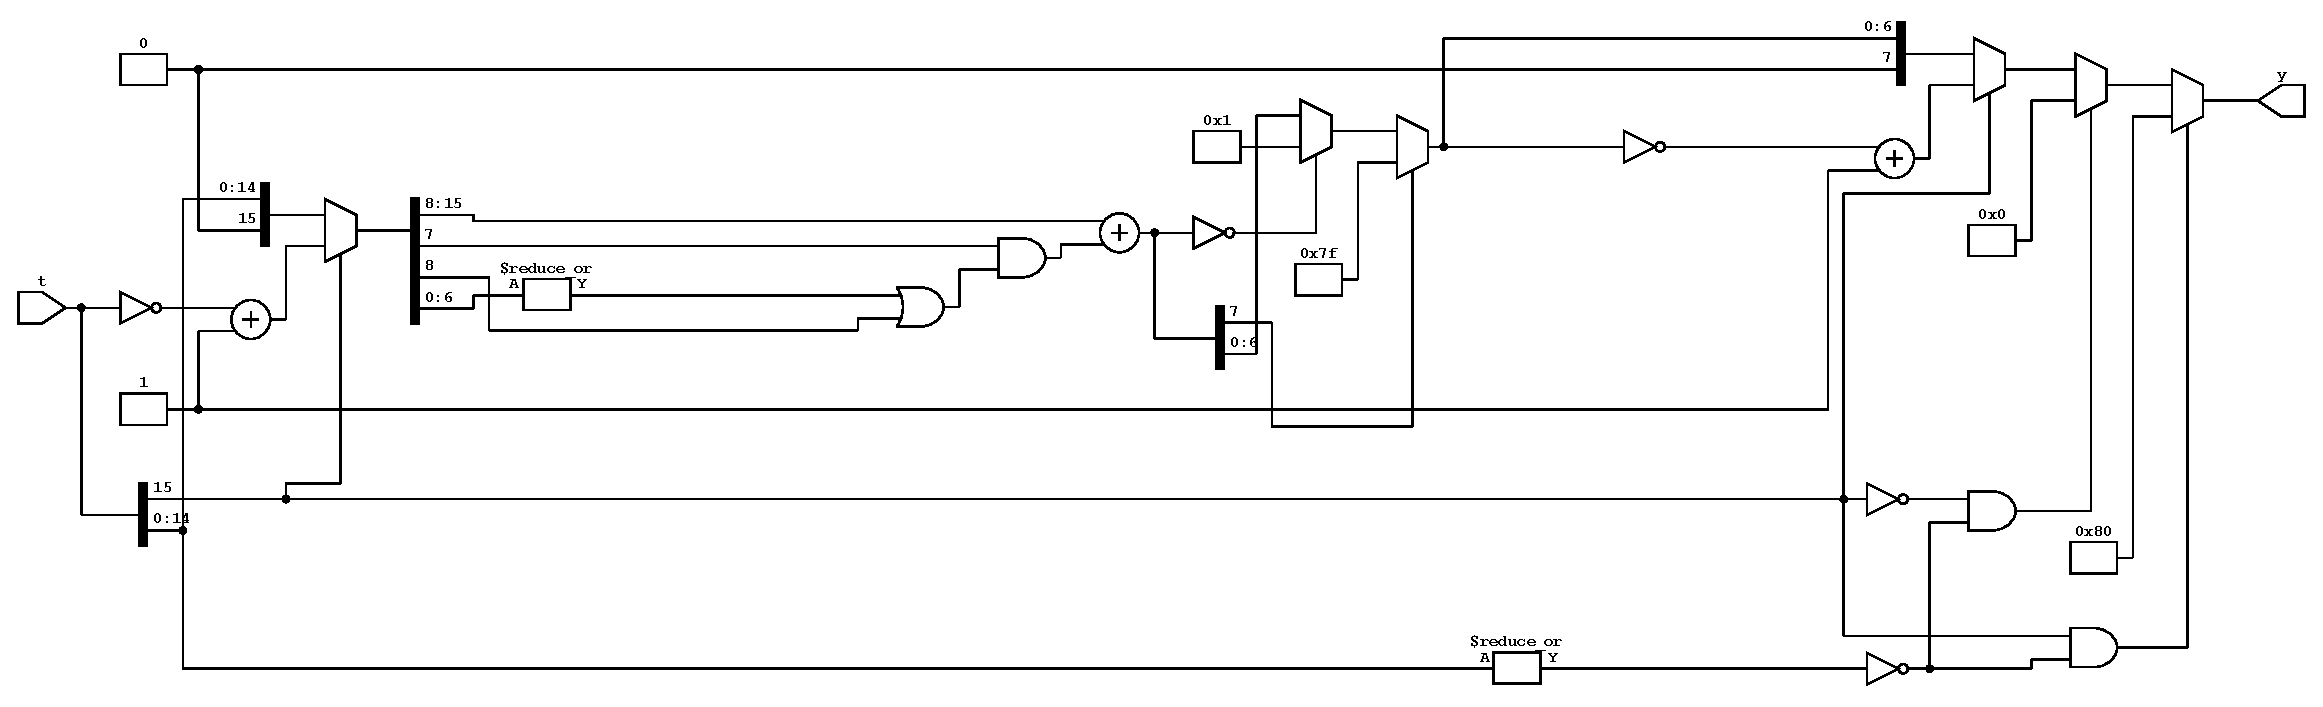
\includegraphics[width=\linewidth]{../img/takum_ncvt.pdf}
\caption{Esquemático do \code{takum\_ncvt} (16 para 8 bits), o módulo do \code{vncvt.t.t}. Da esquerda
para a direita: a negação condicional da entrada (inversor e somador), a separação em metade de cima
(\code{8:15}), bit de guarda (\code{7}) e resto (\code{0:6}), o somador que arredonda, os dois
multiplexadores de saturação (constantes \code{0x7f} e \code{0x1}) e a negação final. Não há
decodificador.}
\end{figure}

\begin{figure}[H]
\centering
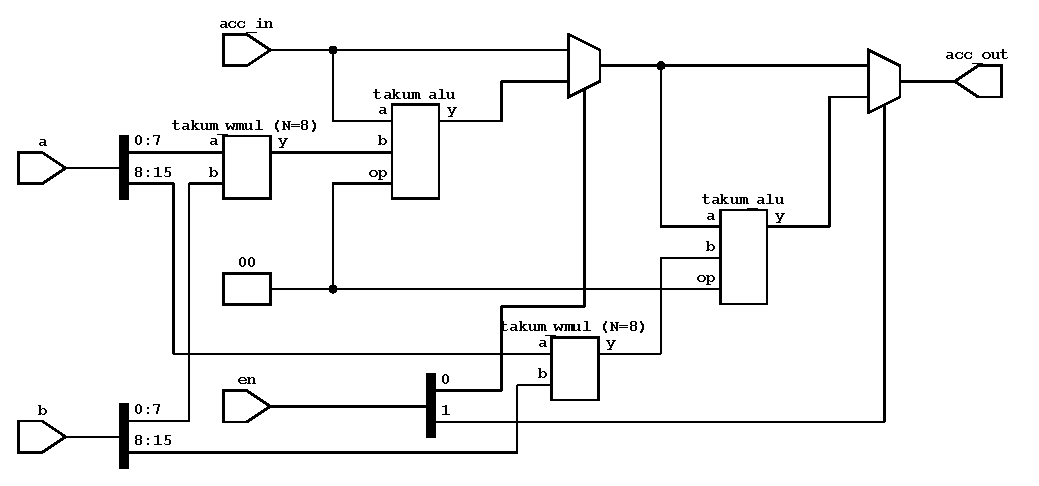
\includegraphics[width=0.92\linewidth]{../img/takum_dot.pdf}
\caption{Esquemático do \code{takum\_dot} com duas pistas. Cada pista tem um \code{takum\_wmul} (produto
alargado) e um \code{takum\_alu} usado como somador (\code{op} fixo em \code{00}); o multiplexador depois
de cada somador escolhe, pelo bit de \code{en}, entre o acumulador novo e o antigo. O acumulador passa de
uma pista para a seguinte: é a cadeia da Figura~2, agora tirada do código.}
\end{figure}

\begin{figure}[H]
\centering
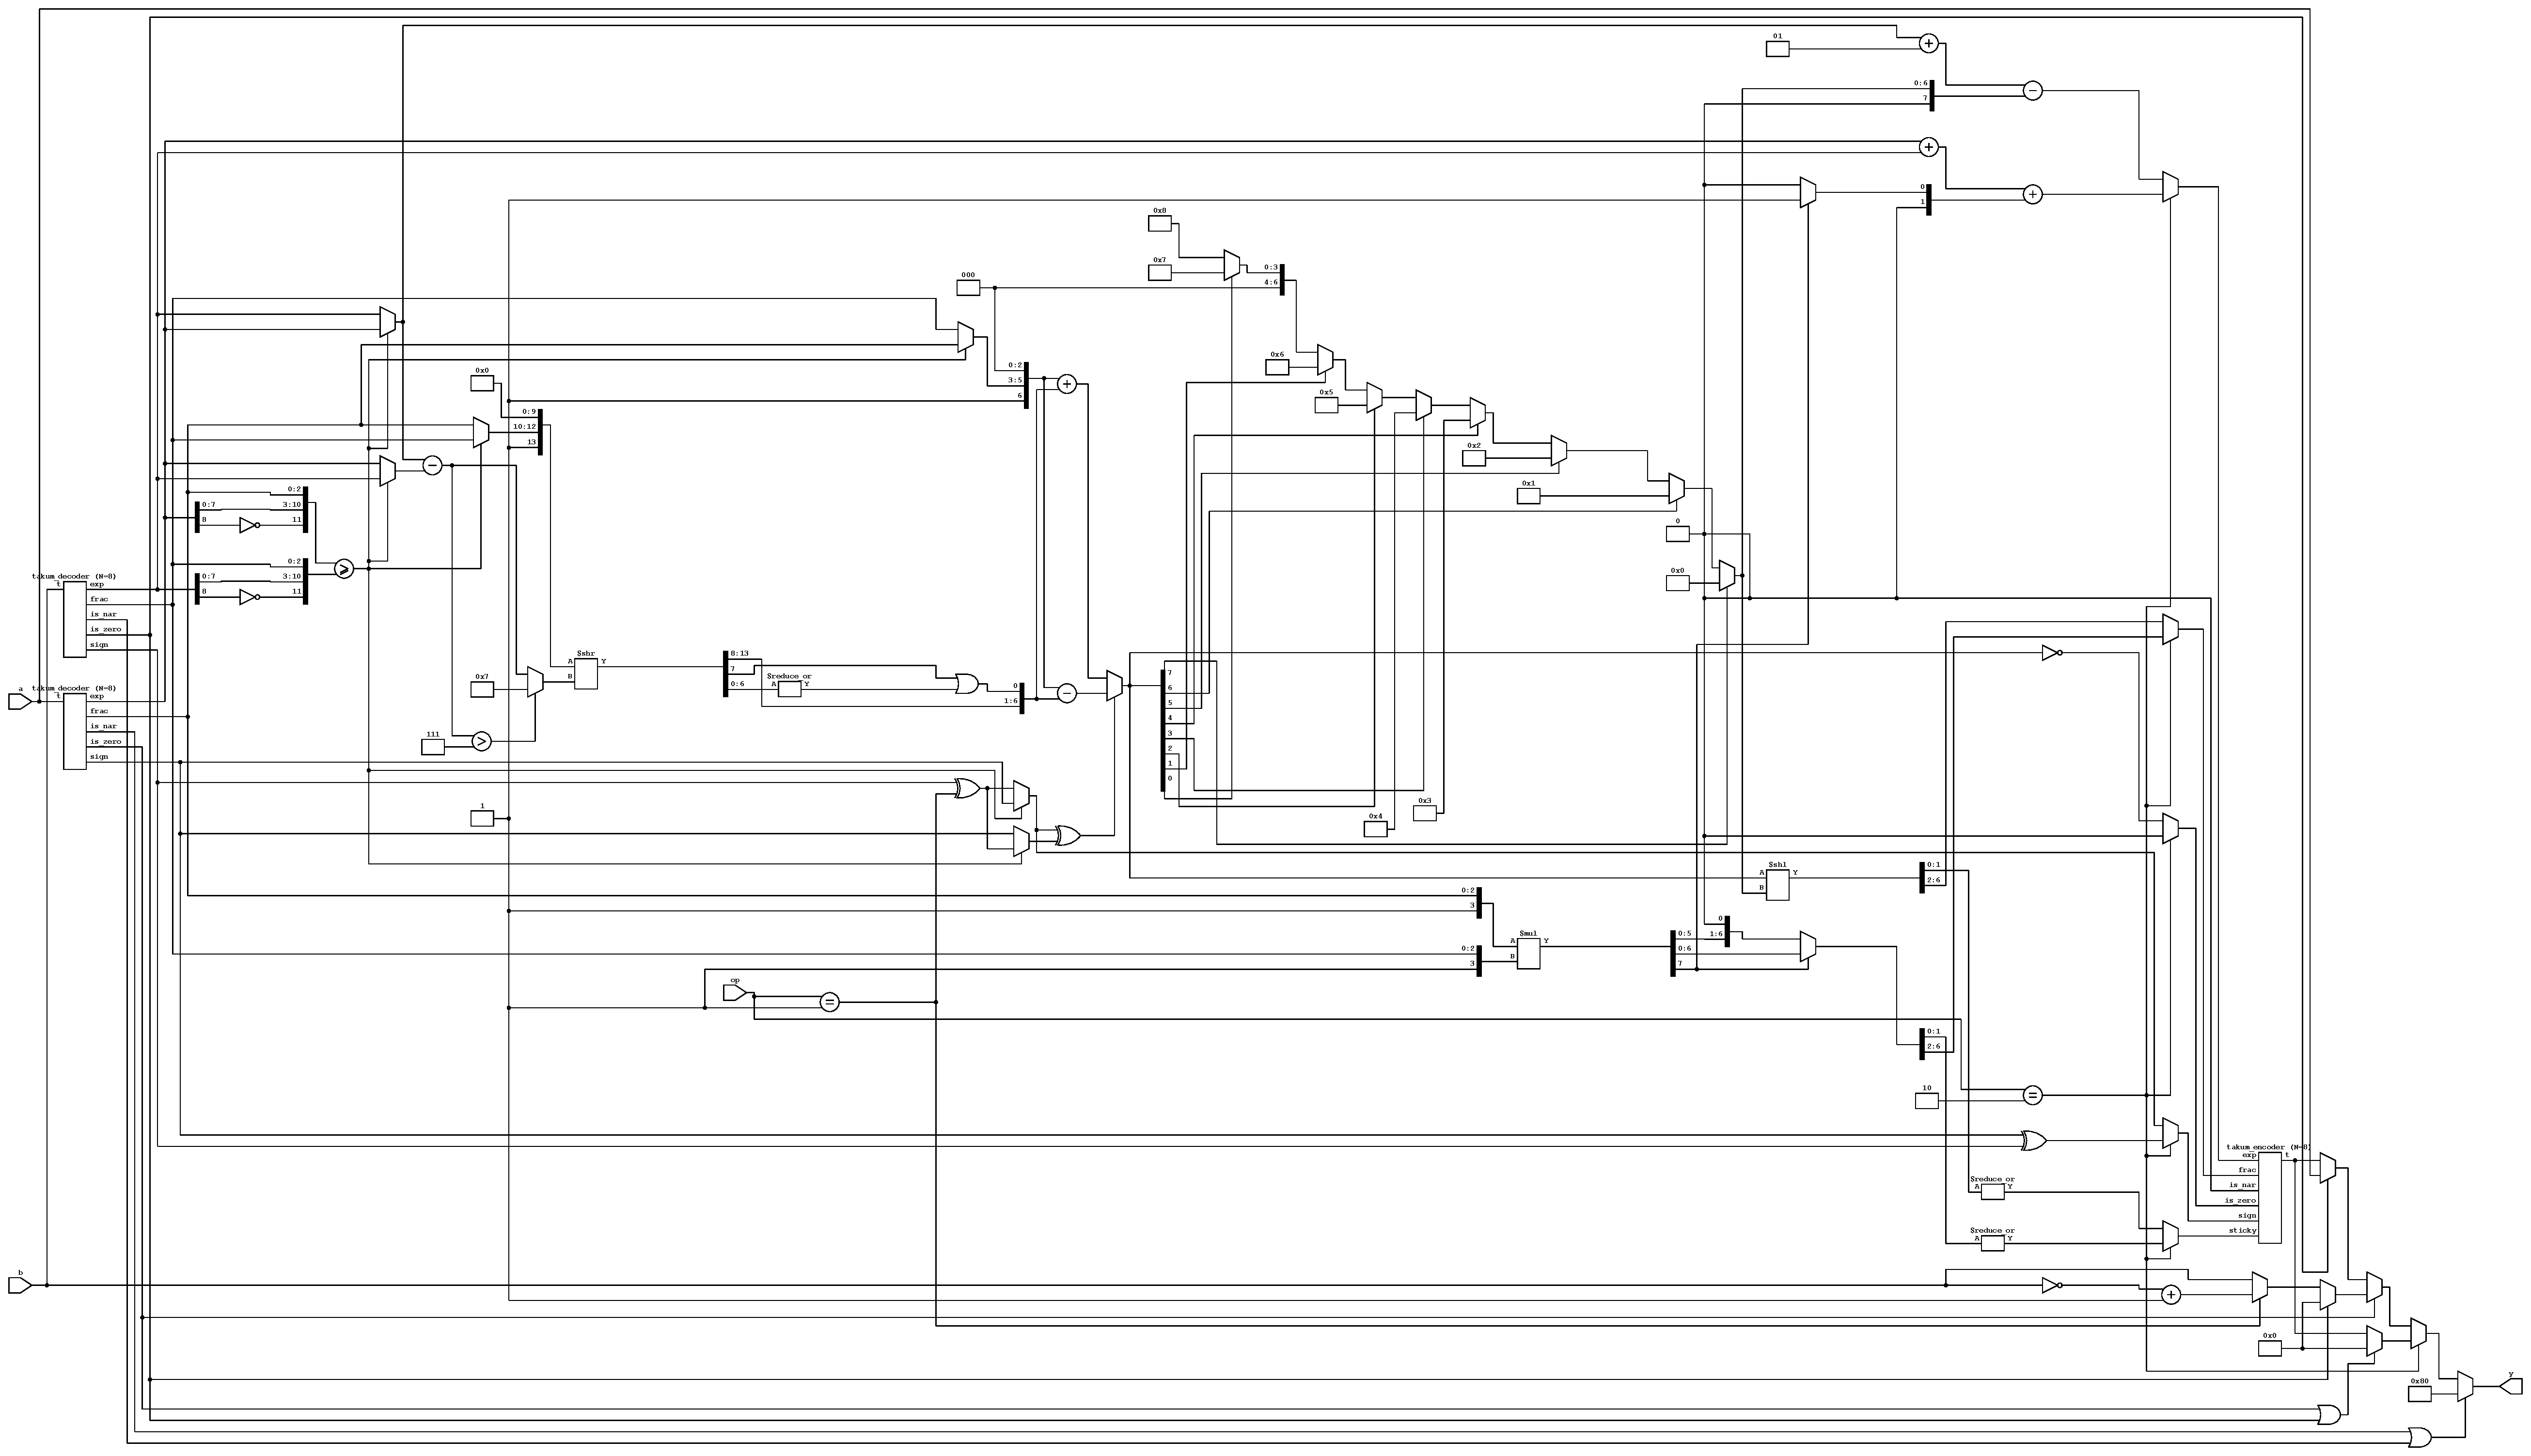
\includegraphics[width=\linewidth]{../img/takum_alu.pdf}
\caption{Esquemático da \code{takum\_alu} de 8 bits. É denso demais para ler impresso; a imagem é
vetorial, e o arquivo \code{docs/img/takum\_alu.svg} pode ser ampliado à vontade. À esquerda, os dois
decodificadores; no centro, em cima, o alinhamento e a soma (\code{\$shr} é o deslocador de alinhamento) e
a cadeia de multiplexadores que conta os zeros à esquerda; embaixo, o multiplicador (\code{\$mul}); à
direita, o codificador e os multiplexadores dos casos especiais.}
\end{figure}

Também são gerados os esquemáticos de \code{takum\_hdr\_dec}, \code{takum\_decoder},
\code{takum\_encoder} e \code{takum\_wmul}.

\subsection{Formas de onda: o circuito funcionando}

O comando \code{make waves2} simula o testbench \code{tb/tb\_demo2.v}, que aplica um caso novo a cada
10~ns, e desenha o que cada sinal valeu ao longo do tempo. Cada caixa mostra o padrão de bits em
hexadecimal e, depois do sinal de igual, o número que ele representa. A última linha, em itálico, é um
comentário nosso; todas as outras são sinais do circuito.

\begin{figure}[H]
\centering
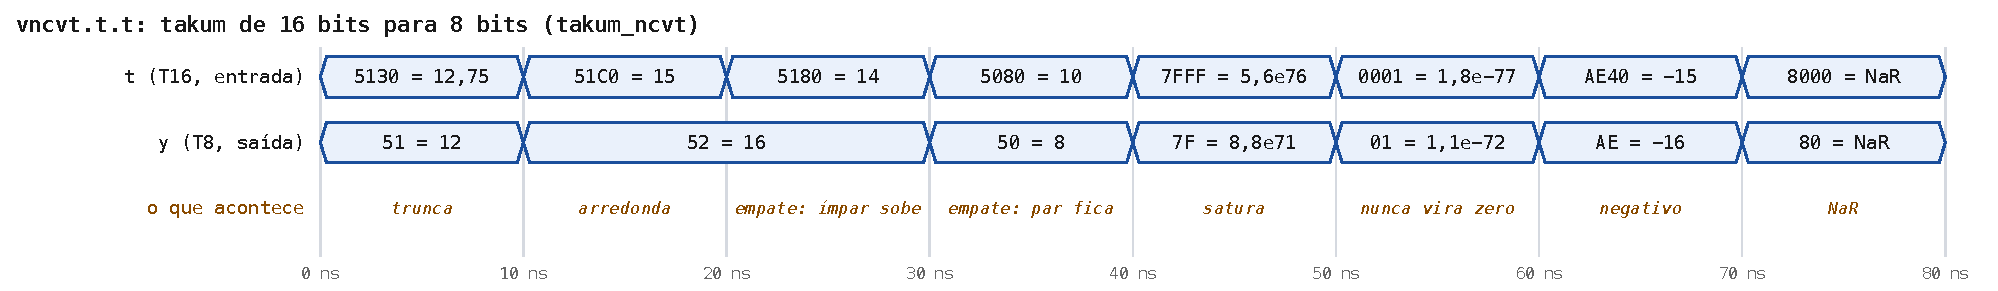
\includegraphics[width=\linewidth]{../img/ondas-fase2-ncvt.pdf}
\caption{\code{vncvt.t.t} em oito situações. Note os dois empates: 14 fica exatamente entre 12 e 16 e vai
para 16 porque a palavra \code{51} é ímpar; 10 fica entre 8 e 12 e vai para 8 porque \code{50} é par.}
\end{figure}

\begin{figure}[H]
\centering
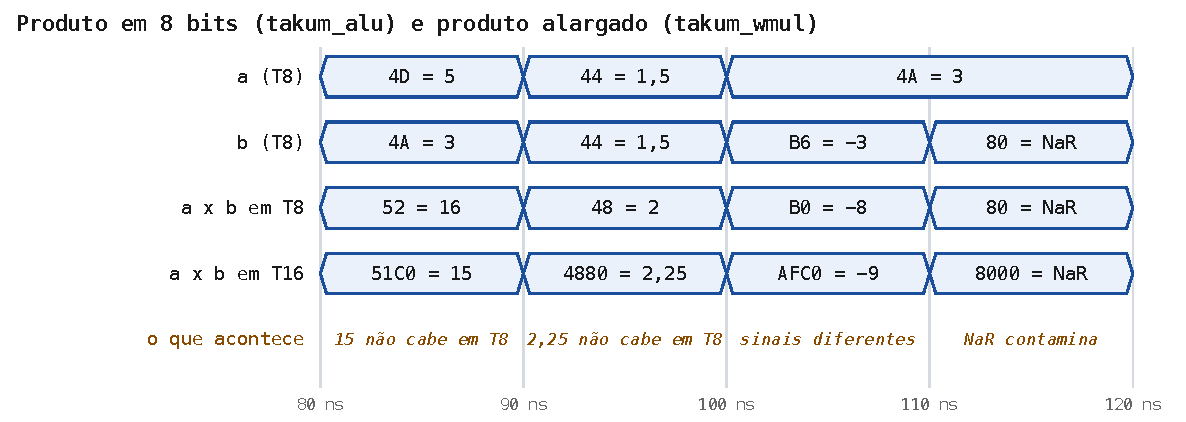
\includegraphics[width=0.72\linewidth]{../img/ondas-fase2-wmul.pdf}
\caption{O mesmo produto em 8 bits e alargado para 16. É o exemplo da Seção~4: $5\times3$ dá 16 em T8 e
15, exato, em T16.}
\end{figure}

\begin{figure}[H]
\centering
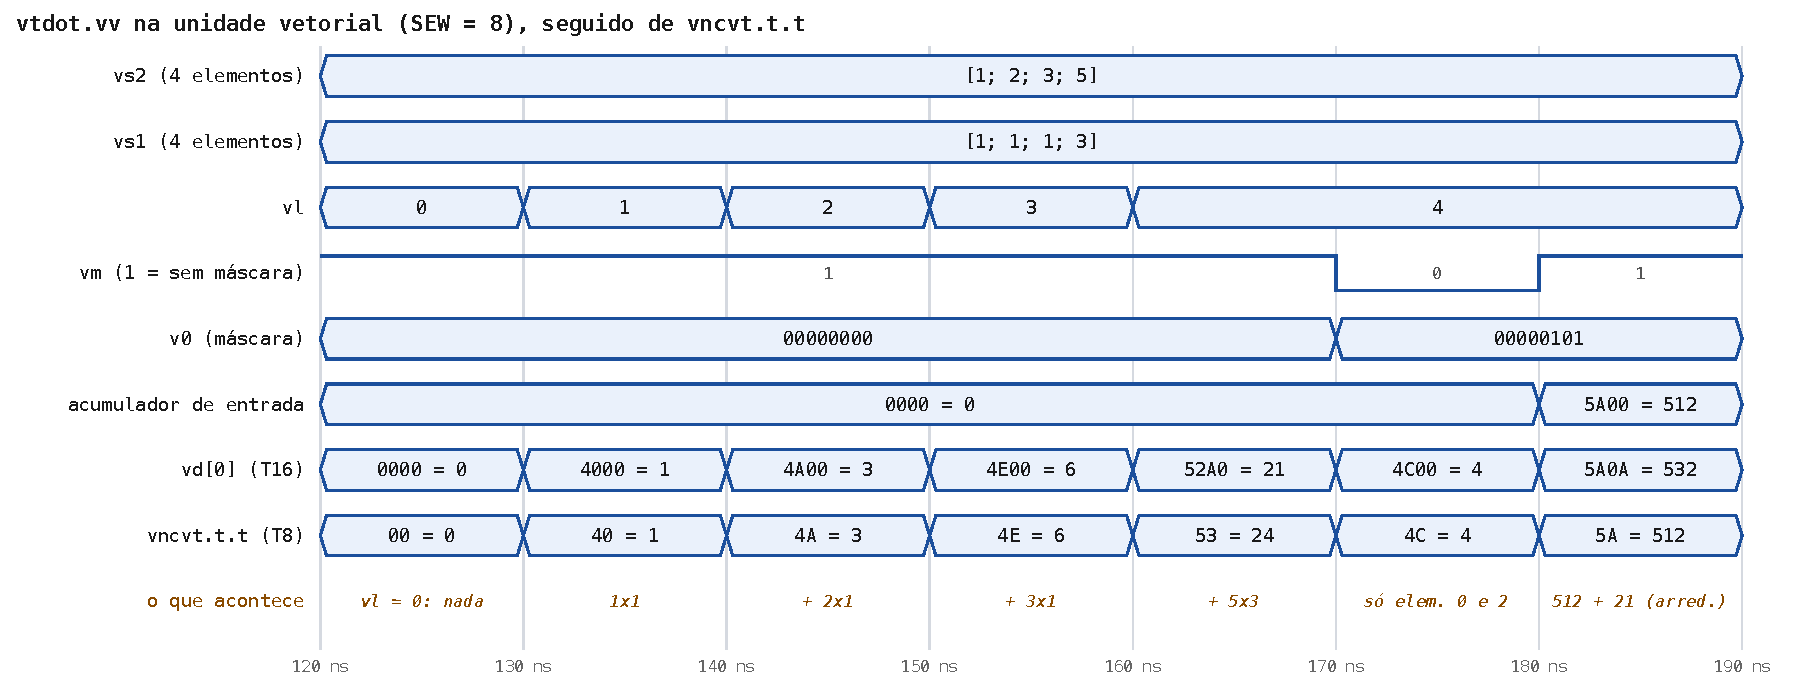
\includegraphics[width=\linewidth]{../img/ondas-fase2-vtdot.pdf}
\caption{\code{vtdot.vv} na unidade vetorial, com $vs2=[1;2;3;5]$ e $vs1=[1;1;1;3]$. Aumentando
\code{vl}, o acumulador \code{vd[0]} soma um produto por vez: 1, 3, 6, 21. Com a máscara \code{101}, só os
elementos 0 e 2 entram ($1+3=4$). No último caso o acumulador começa em 512 e o resultado é 532, não 533:
perto de 512 um T16 anda de 2 em 2. A linha de baixo é o \code{vncvt.t.t} do acumulador: 21 vira 24 em
T8.}
\end{figure}

As ondas da Fase~1 (decodificador e codificador) também estão em \code{docs/img/}, nos arquivos cujo
nome começa por \code{ondas-parte1} e \code{ondas-parte2}. Quem quiser navegar pelos sinais internos pode
abrir a simulação da Fase~1 no GTKWave com \code{make waves}.

%======================================================================
\section{Como sabemos que o hardware está certo}

\paragraph{O oráculo.} \code{tb/takum\_oracle.py} é um segundo cálculo, independente. Ele decodifica cada
operando para uma fração exata (\code{Fraction} do Python, sem arredondamento nenhum), faz a conta exata e
só então procura o takum mais próximo. Não compartilha código nem método com o Verilog; se os dois
concordam, é muito improvável que estejam errados do mesmo jeito.

\paragraph{Os testes.} Um script gera arquivos com entradas e respostas esperadas, e os \emph{testbenches}
comparam o hardware simulado (Icarus Verilog) com elas.

\begin{center}
\begin{tabular}{lr}
\toprule
Teste & Casos \\
\midrule
Decodificador, codificador, ida e volta & 855\,408 \\
ALU de 8 bits: \textbf{todos} os $256\times256$ pares, nas 3 operações & 196\,608 \\
ALU de 16 e de 32 bits: casos de borda e aleatórios (cada) & 109\,923 \\
\code{vncvt.t.t}: \textbf{todas} as palavras de 16 bits, e amostras de 32 e 64 & 105\,794 \\
Produto alargado: \textbf{todos} os pares de 8 bits, e amostras de 16 e 32 & 138\,818 \\
Unidade vetorial: 5 instruções, com \code{vl} e máscara variados (por largura) & 5\,000 \\
\bottomrule
\end{tabular}
\end{center}

Em 8 bits o teste é exaustivo: não existe entrada não testada. Em 16 e 32 bits o espaço é grande demais
($2^{32}$ e $2^{64}$ pares), então a amostra concentra-se onde os erros costumam se esconder: fronteiras
de regime, números vizinhos (cancelamento na subtração), empates de arredondamento.

\paragraph{Uma terceira opinião: a libtakum.} O hardware e o oráculo foram escritos por nós, a partir da
mesma leitura do artigo de Hunhold. Se tivéssemos entendido algo errado, os dois poderiam errar igual e
concordar. Para afastar esse risco, comparamos os mesmos vetores com a \emph{libtakum}, a biblioteca em C
publicada pelo próprio autor do formato (\code{make libtakum} baixa, compila e compara).

\begin{center}
\begin{tabularx}{\linewidth}{Xrl}
\toprule
O que foi comparado & Vetores & Resultado \\
\midrule
Decodificar e recodificar (T8 e T16 completos; T32 amostrado) & 165\,921 & idênticos \\
Soma, subtração e produto em T8 (todos os pares) & 196\,608 & idênticos \\
Soma, subtração e produto em T16 & 109\,923 & idênticos \\
Soma, subtração e produto em T32 & 109\,923 & 16 diferem no último bit \\
\code{vncvt.t.t} (T16$\to$T8 completo e amostras maiores) & 105\,794 & idênticos \\
Produto alargado (T8 completo, T16, T32) & 138\,818 & idênticos \\
\bottomrule
\end{tabularx}
\end{center}

Dos 826\,987 vetores, 16 diferem, todos produtos em T32. A explicação está na libtakum, não no nosso
código: ela faz as contas em \code{double}, que guarda 53 bits, e o produto de dois T32 pode precisar de
56. Ela arredonda uma vez para caber no \code{double} e outra para virar takum, e nesses 16 casos o
arredondamento duplo erra o último bit. Conferimos cada um com frações exatas: em todos, o resultado
exato está mais perto do nosso valor.

Um detalhe prático: no Mac com processador ARM em que trabalhamos, a suíte de testes da própria libtakum
falha (por exemplo, o 3 é codificado como 2). Por isso o \code{make libtakum} a compila para x86-64 e a
executa pela camada de tradução do sistema; assim compilada, ela se comporta como esperado.

\paragraph{Os testes pegam erros?} Um teste que sempre passa pode ser um teste que não testa. Para
conferir, estragamos o hardware de propósito, 13 vezes, um defeito por vez: tirar o bit \emph{sticky},
esquecer a regra do empate, não normalizar o produto, ignorar a máscara, acumular o produto escalar na
ordem errada, e assim por diante. \textbf{Os testes acusaram os 13.} A lista está em
\code{docs/04-entrega1-alu.md} e \code{docs/05-entrega2.md}.

%======================================================================
\section{O simulador}

\subsection{Para que serve}

O hardware faz uma operação. Para medir erro e contar instruções em um problema real, é preciso rodar
\emph{programas}: laços, leituras de memória, configuração do vetor. O enunciado permite um simulador
funcional para isso, e o escrevemos em Python (\code{sim/}).

Ele funciona como um processador simplificado:
\begin{enumerate}[nosep]
  \item o \textbf{montador} (\code{isa.py}) traduz o texto do programa em palavras de 32 bits;
  \item a \textbf{máquina} (\code{rvv.py}) guarda registradores e memória, busca a palavra apontada pelo
        PC, \textbf{decodifica a partir dos bits} e executa;
  \item a cada instrução, um contador é incrementado.
\end{enumerate}

Ele conhece um pedaço pequeno do RISC-V: aritmética inteira e desvios para escrever laços; da RVV, a
configuração (\code{vsetvli}), cargas e armazenamentos, a carga indexada e as instruções de ponto
flutuante usadas; e as cinco da Zvtakum.

\paragraph{De onde vêm as contas.} As operações takum chamam o mesmo oráculo que verifica o hardware. As
operações IEEE usam um modelo nosso, genérico, que serve para qualquer formato binário (FP8, binary16,
bfloat16, binary32, binary64, binary128) e também faz a conta exata antes de arredondar. Ele registra os
\emph{flags} de exceção, como um processador real.

\paragraph{O simulador confere com o hardware?} Sim, e isso é testado. Os $15\,000$ vetores usados para
testar a unidade vetorial em Verilog são reexecutados no simulador como instruções codificadas, e o
resultado tem de ser idêntico. O modelo IEEE é conferido contra o ponto flutuante do próprio computador em
$160\,000$ casos.

\subsection{O programa de teste: matriz esparsa vezes vetor}

Uma matriz \emph{esparsa} tem quase todos os elementos nulos, e só os não nulos são guardados. O formato
usual é o CSR (\emph{Compressed Sparse Row}), com três vetores. Para a matriz
\[
A=\begin{pmatrix} 5 & 0 & 0 & 1\\ 0 & 2 & 0 & 0\\ 0 & 3 & 4 & 0 \end{pmatrix}
\qquad
\begin{aligned}
\texttt{val} &= [5,\,1,\,2,\,3,\,4] &&\text{os não nulos, linha a linha}\\
\texttt{col} &= [0,\,3,\,1,\,1,\,2] &&\text{a coluna de cada um}\\
\texttt{rowptr} &= [0,\,2,\,3,\,5] &&\text{onde cada linha começa em \texttt{val}}
\end{aligned}
\]
Calcular $y=Ax$ é fazer, para cada linha $i$, o produto escalar dos seus não nulos com os elementos
correspondentes de $x$: $y_i=\sum_k \texttt{val}[k]\cdot x[\texttt{col}[k]]$. É por isso que o
\code{vtdot.vv} importa.

O miolo do programa em assembly, para elementos de 16 bits (arquivo \code{sim/kernels.py}):

\begin{lstlisting}
inner:
  vsetvli    t3, t2, e16, m1, ta, ma   # quantos elementos cabem nesta volta (vl)
  vle32.v    v8, (a2)                  # carrega as colunas (já em bytes)
  vle16.v    v1, (a3)                  # carrega os valores da linha
  vluxei32.v v2, (a4), v8              # busca x[col] na memória (carga indexada)
  vtdot.vv   v4, v1, v2                # acumulador T32 em v4[0] += v1 . v2
  ...                                  # avança os ponteiros; repete se sobrou
done:
  vncvt.t.t  v5, v4                    # T32 -> T16
  vse16.v    v5, (a5)                  # grava y[i]
\end{lstlisting}

O \code{vsetvli} é o que torna o laço independente do tamanho do registrador: ele recebe quantos
elementos faltam e devolve quantos cabem. O mesmo programa roda com vetores de 64 ou de 512 bits.

\subsection{As três versões comparadas}

\begin{center}
\begin{tabularx}{\linewidth}{l>{\raggedright\arraybackslash}p{4.6cm}X}
\toprule
Nome & Instruções do miolo & Observação \\
\midrule
T8, T16, T32 & \code{vtdot.vv}; \code{vncvt.t.t} no fim & a nossa extensão \\
FP8, FP16, FP32 & \code{vfmul.vv} e \code{vfredosum.vs} & o jeito usual em RVV: tudo na largura do
  elemento \\
FP8w, FP16w, FP32w & \code{vfwmul.vv}, soma em largura dupla; \code{vfncvt.f.f.w} no fim & IEEE com o
  \emph{mesmo} acúmulo ampliado do \code{vtdot.vv} \\
\bottomrule
\end{tabularx}
\end{center}

A terceira versão existe para a comparação ser justa. Sem ela, não saberíamos se o takum foi melhor por
causa do formato ou só porque acumulou com mais bits. Comparando T com FPw, a única diferença é o formato.

%======================================================================
\section{Os experimentos e o que eles mostram}
\label{sec:exp}

\subsection{O que foi medido}

Usamos nove matrizes. Quatro são \textbf{geradas} por programa, com semente fixa (sempre saem iguais), e
cada uma foi desenhada para provocar um comportamento:

\begin{center}
\begin{tabularx}{\linewidth}{lX}
\toprule
Nome & O que é e por que está aqui \\
\midrule
\code{poisson} & A matriz da equação de Poisson em uma malha $16\times16$ (4 na diagonal, $-1$ nos
  vizinhos), aplicada a uma função suave. Em cada linha, números parecidos se subtraem: é o teste de
  \emph{cancelamento} \\
\code{gauss} & Aleatória, 10 não nulos por linha, valores com distribuição normal em torno de zero. Todos
  os números têm tamanho parecido: \emph{faixa estreita} \\
\code{wide} & Mesma estrutura, mas com magnitudes de $2^{-10}$ a $2^{10}$ na matriz e de $2^{-6}$ a
  $2^{6}$ no vetor: \emph{faixa larga} \\
\code{mlp} & Uma camada de rede neural \emph{podada}: $256\times512$, 90\% de zeros, entrada depois de uma
  ReLU. É o ``kernel de aprendizado de máquina'' do enunciado \\
\bottomrule
\end{tabularx}
\end{center}

As outras cinco são \textbf{reais}: vêm de problemas de engenharia e estão em um repositório público, o
\emph{Matrix Market} do NIST. Quatro pertencem à coleção Harwell-Boeing, usada há décadas para testar
programas de álgebra linear, e são pequenas. A quinta, \code{memplus}, é a \textbf{matriz grande} do
experimento: tem quase 70 vezes mais linhas que as geradas. Elas servem para responder à pergunta ``e com dados que vocês não escolheram?''.

\begin{center}
\begin{tabularx}{\linewidth}{lX}
\toprule
Nome & De onde vem \\
\midrule
\code{nos4} & Análise estrutural de uma viga. Valores todos entre $2^{-6}$ e $2^{-1}$: faixa estreita,
  abaixo de 1 \\
\code{bus494} & Rede elétrica de 494 barras (arquivo \code{494\_bus}). Valores de $2^{-3}$ a $2^{14}$ \\
\code{west0479} & Engenharia química: modelo de uma coluna de destilação. Valores de $2^{-21}$ a
  $2^{18}$ \\
\code{bcsstk05} & Matriz de rigidez de uma estrutura. Valores de $2^{-31}$ a $2^{22}$: os maiores passam
  de três milhões \\
\code{memplus} & Simulação de um circuito de memória de computador: $17\,758\times17\,758$, com
  $126\,150$ elementos. Valores de $2^{-86}$ a $2^{0}$: muitos são minúsculos \\
\bottomrule
\end{tabularx}
\end{center}

\begin{table}[H]
\centering
\caption{As nove matrizes. A última coluna é a faixa dos módulos dos elementos não nulos.}
\smallskip
\begin{tabular}{lcrrc}
\toprule
Matriz & Dimensão & Não nulos & Por linha & Faixa de $|a_{ij}|$\\
\midrule
\MATTABLE
\bottomrule
\end{tabular}
\end{table}

Nas matrizes reais o vetor $x$ é sorteado (distribuição normal, semente fixa). O arquivo
\code{data/matrixmarket/LEIAME.md} lista o endereço de origem de cada matriz. A função \code{read\_mm} de
\code{sim/bench.py} lê o formato do repositório; nas matrizes simétricas, que guardam só metade dos
elementos, ela espelha a outra metade. Rodar a \code{memplus} em todos os formatos leva cerca de um
minuto; por ter muitas linhas, seus arquivos de curva guardam 500 pontos igualmente espaçados em vez de
todas as linhas (o resumo usa todas).

O procedimento, para cada matriz e cada formato:
\begin{enumerate}[nosep]
  \item os dados (em precisão dupla) são arredondados para o formato;
  \item o programa da seção anterior calcula $y$ no simulador;
  \item cada $y_i$ é comparado com a \emph{referência}: a mesma conta em precisão quádrupla (binary128,
        113 bits de precisão), feita sobre os dados originais.
\end{enumerate}
A medida é o \textbf{erro relativo} $|y_i-\text{ref}_i|/|\text{ref}_i|$. Um erro de $10^{-3}$ significa
três algarismos corretos. Como a referência usa os dados \emph{antes} do arredondamento, o erro inclui o
custo de não conseguir representar bem as entradas, que faz parte da qualidade de um formato.

\subsection{Como ler o gráfico}

A Figura~\ref{fig:cdf} mostra, para cada matriz, a \emph{distribuição acumulada} do erro: a curva diz que
fração das linhas teve erro menor ou igual ao valor do eixo horizontal. \textbf{Quanto mais à esquerda
a curva, melhor.} Linha contínua é takum; tracejada é o IEEE com acúmulo ampliado; a cor indica a largura.
Uma curva tracejada que para antes de chegar a 1 indica que o restante das linhas deu infinito ou NaN.

\begin{figure}[H]
\centering
\begin{tikzpicture}
\begin{groupplot}[
  group style={group size=3 by 3, horizontal sep=5mm, vertical sep=11mm, ylabels at=edge left,
               yticklabels at=edge left, xlabels at=edge bottom},
  width=0.38\textwidth, height=48mm,
  xmode=log, xmin=1e-10, xmax=1e2, ymin=0, ymax=1,
  xtick={1e-10,1e-8,1e-6,1e-4,1e-2,1e0,1e2},
  xticklabels={,$10^{-8}$,,$10^{-4}$,,$10^{0}$,},
  yticklabels={,0,{0,2},{0,4},{0,6},{0,8},1},
  xlabel={erro relativo}, ylabel={fração das linhas},
  grid=major, grid style={black!12},
  tick label style={font=\scriptsize}, label style={font=\footnotesize}, title style={font=\footnotesize, yshift=-1.5mm},
  cycle list={}, every axis plot/.append style={line width=0.9pt},
  legend style={font=\scriptsize, legend columns=6, /tikz/every even column/.append style={column sep=3mm}}]
\matplot{poisson}
\matplot{gauss}
\matplot{wide}
\matplot{mlp}
\matplot{nos4}
\matplot{bus494}
\matplot{west0479}
\matplot{bcsstk05}
\matplot[legend to name=cdfleg]{memplus}
\legend{T8, FP8w, T16, FP16w, T32, FP32w}
\end{groupplot}
\end{tikzpicture}\\[1.5mm]
\pgfplotslegendfromname{cdfleg}
\caption{Distribuição acumulada do erro relativo de $y=Ax$. As quatro primeiras matrizes são geradas; as
cinco últimas, reais.}
\label{fig:cdf}
\end{figure}

\begin{table}[H]
\centering
\caption{Erro relativo mediano nas matrizes geradas (metade das linhas erra menos que isto). Em negrito,
o melhor de cada largura.}
\label{tab:err}
\smallskip
\begin{tabular}{lcccc}
\toprule
 & poisson & gauss & wide & mlp\\
\midrule
\ERRTABLESYN
\bottomrule
\end{tabular}
\end{table}

\begin{table}[H]
\centering
\caption{Erro relativo mediano nas matrizes reais. O símbolo $\infty$ indica que mais da metade das
linhas não deu um número.}
\label{tab:errreal}
\smallskip
\small
\begin{tabular}{lccccc}
\toprule
 & nos4 & bus494 & west0479 & bcsstk05 & memplus\\
\midrule
\ERRTABLEREAL
\bottomrule
\end{tabular}
\end{table}

\begin{table}[H]
\centering
\caption{Quantas linhas deram infinito ou NaN (núcleos com acúmulo ampliado). Nas matrizes que não
aparecem, nenhuma.}
\smallskip
\begin{tabular}{lcccc}
\toprule
 & wide & bus494 & west0479 & bcsstk05\\
\midrule
Linhas da matriz & 256 & 494 & 479 & 153\\
\midrule
FP8w & \FPEIGHTBAD & \NFBUS & \NFWEST & \NFBCS\\
FP16w & 0 & 0 & \NFWESTH & \NFBCSH\\
FP32w & 0 & 0 & 0 & 0\\
T8, T16, T32 & 0 & 0 & 0 & 0\\
\bottomrule
\end{tabular}
\end{table}

\subsection{O que aconteceu, largura por largura}

Tudo se explica pela tabela de bits de fração da Seção~3 e pela faixa de valores de cada matriz.

\paragraph{32 bits: o takum ganha sempre.} De \RATA{} a \RATB{} vezes menos erro que o FP32w, nas nove
matrizes. Os números desses testes ficam quase todos em faixas com $r\le3$, em que o T32 tem de 24 a 27
bits de fração; o binary32 tem 23 em qualquer lugar. Cada bit a mais divide o erro por dois. O menor
ganho é em \code{bcsstk05}: seus valores chegam a $2^{22}$, onde $r=4$ e o T32 fica com os mesmos 23
bits.

\paragraph{16 bits: depende dos dados.} Há três situações.
\begin{itemize}[nosep]
  \item \emph{Dados perto de 1} (\code{poisson}, \code{gauss}, \code{mlp}, \code{nos4} e a maior parte de
        \code{west0479}): o T16 tem 10 ou 11 bits e ganha.
  \item \emph{Faixa moderadamente larga} (\code{wide}, \code{bus494} e \code{memplus}): o T16
        \textbf{perde}. Em \code{wide}, \WIDET{} contra \WIDEF{}; em \code{bus494}, \BUST{} contra
        \BUSF{}; em \code{memplus}, \MEMTS{} contra \MEMFS{}. Números em torno de $2^{10}$ ou de
        $2^{-10}$ caem na faixa $r=3$, com 8 bits, e o binary16 tem 10. É o preço do afunilamento, e
        fizemos questão de mostrá-lo.
  \item \emph{Faixa além do binary16}, cujo maior número é $65\,504$: em \code{bcsstk05}, o binary16 deu
        infinito ou NaN em \NFBCSH{} das 153 linhas; em \code{west0479}, em \NFWESTH{} das 479. O T16
        respondeu em todas, com erro mediano de \BCSTSIXTEEN{} em \code{bcsstk05}.
\end{itemize}

\paragraph{8 bits: menos precisão, muito mais faixa.} Quando os dados cabem na faixa do FP8, ele é mais
preciso que o T8, de 1,5 a 3 vezes na mediana. O motivo está na tabela da Seção~3: o T8 só tem 3 bits de
fração entre 0,5 e 2, e a matriz \code{nos4}, com todos os valores abaixo de 0,5, cai onde ele tem 2 ou 1.
Os dois são inúteis em \code{poisson}: com tão poucos bits, o cancelamento deixa só ruído.

Mas a faixa do FP8 acaba em 240, e isso aparece em \textbf{quatro das nove matrizes}, incluindo três das
cinco reais: ele devolveu infinito ou NaN em \FPEIGHTBAD{} das 256 linhas de \code{wide}, \NFBUS{} das
494 de \code{bus494}, \NFWEST{} das 479 de \code{west0479} e em \emph{todas} as \NFBCS{} de
\code{bcsstk05}. O T8 devolveu um número em todas as linhas de todas as matrizes. Em \code{bcsstk05} seu
erro mediano é grande (\BCSTEIGHT), mas é uma resposta; um NaN não é.

A \code{memplus} mostra o limite na outra ponta. Seus valores chegam a $2^{-86}$, muito abaixo do menor
número do FP8 ($2^{-9}$), que os arredonda para zero (\emph{underflow}). Não aparece infinito nem NaN, mas
o FP8w erra 100\% ou mais em \MEMFEBAD{} das \MEMROWS{} linhas; o T8, em \MEMTEBAD. Na mediana, porém, o
FP8w continua melhor (\MEMFE{} contra \MEMTE).

\paragraph{O que as matrizes reais mudaram.} Só com as geradas, a conclusão para 8 bits seria ``precisão
parecida''. Com dados reais ficou claro que o FP8 é mais preciso dentro da faixa e que sair da faixa é
comum, não um caso construído. Para 16 bits, apareceu o terceiro cenário, o do estouro do binary16, que as
matrizes geradas não mostravam. Para 32 bits, a conclusão se manteve.

\paragraph{E a matriz grande?} A \code{memplus} tem 17\,758 linhas contra 100 a 494 das outras reais, e
\textbf{confirmou o padrão} em vez de mudá-lo: T32 à frente (\MEMTT{} contra \MEMFT), T16 atrás do
binary16 por menos de 2 vezes, T8 atrás do FP8 na mediana e à frente nos casos extremos. Isso indica que
as conclusões não dependiam de as matrizes serem pequenas.

\paragraph{Quanto vale o acúmulo ampliado.} Refizemos a conta takum sem ele (\code{vtmul} e \code{vtadd}
na largura do elemento): o erro mediano cresce de 1,2 a 2,3 vezes. Com ele, fora \code{poisson}, o
resultado fica a menos de 3 vezes do melhor possível, que é a referência arredondada diretamente para o
formato. Ou seja, quase todo o erro que resta vem de arredondar as \emph{entradas}, não da conta.

\subsection{Contagem de instruções}
\label{sec:instr}

O simulador conta cada instrução executada. Por volta do laço interno:

\begin{center}
\begin{tabularx}{\linewidth}{lcX}
\toprule
Versão & Por volta & Por quê \\
\midrule
Zvtakum & 11 & \code{vtdot.vv} multiplica e acumula \\
IEEE simples (FP) & 12 & \code{vfmul} e depois \code{vfredosum} \\
IEEE com alargamento (FPw) & 13 & \code{vfwmul}, um \code{vsetvli} para mudar a largura e
  \code{vfredosum} \\
\bottomrule
\end{tabularx}
\end{center}

A linha do FPw mostra uma dor real da RVV: os produtos alargados têm outra largura de elemento, e mudar de
largura exige reconfigurar o vetor a cada volta. O \code{vtdot.vv} entrega a soma alargada sem mexer na
configuração.

\begin{table}[H]
\centering
\caption{Instruções executadas no produto completo, com elementos de 16 bits e registradores vetoriais de
128 bits. A matriz \code{wide} tem a mesma estrutura de \code{gauss}.}
\smallskip
\begin{tabular}{lrrrrrr}
\toprule
 & Não nulos & & & & \multicolumn{2}{c}{Economia frente a}\\
Matriz & por linha & Zvtakum & FP & FPw & FP & FPw\\
\midrule
\INSTRTABLE
\bottomrule
\end{tabular}
\end{table}

Considerando todas as matrizes e as três larguras, a economia frente ao FPw, que tem a mesma qualidade
numérica, vai de \SAVEWLO\% a \SAVEWHI\%. Frente ao FP simples, de zero a \SAVEPHI\%. O ganho cresce com o
número de não nulos por linha. Quando a linha inteira cabe em uma volta, a instrução que o
\code{vtdot.vv} economiza no laço é gasta no \code{vncvt.t.t} do final, e o resultado é zero: é o que acontece, ou quase, nas matrizes reais, que têm de 3 a 7 não nulos por linha (a exceção é
\code{bcsstk05}, com 16). Na \code{memplus}, o programa takum executa cerca de meio milhão de instruções.
Na \code{mlp}, com 51 por linha, o ganho é o maior.

Uma ressalva honesta: contamos \emph{instruções}, não tempo. Um \code{vtdot.vv} faz mais trabalho que
um \code{vfmul} e, em um processador real, poderia levar mais ciclos.

\subsection{Registradores de controle (CSRs)}

As instruções de ponto flutuante do RISC-V dependem de um registrador de controle, o \code{fcsr}, com
duas partes:
\begin{itemize}[nosep]
  \item \code{frm} (3 bits): qual dos cinco modos de arredondamento usar;
  \item \code{fflags} (5 bits): avisos acumulados (inexato, \emph{underflow}, \emph{overflow}, divisão por
        zero, operação inválida).
\end{itemize}
Toda instrução lê o primeiro e pode escrever no segundo. Para o hardware isso é um incômodo: é estado que
precisa ser salvo e restaurado nas trocas de contexto, e uma dependência entre instruções que atrapalha a
execução fora de ordem.

O takum tem um único modo de arredondamento e avisa de problemas dentro do próprio resultado (o NaR).
\textbf{A Zvtakum não usa nenhum bit do \code{fcsr}.} Nos nossos testes, os programas IEEE levantaram algum
flag em até \FLAGPCT\% das operações, e o FP8 em \code{wide} terminou com quatro dos cinco ligados. Os
programas takum, por construção, zero.

\paragraph{Instruções que deixam de ser necessárias.} Como as palavras takum se ordenam como inteiros:
\begin{itemize}[nosep]
  \item as seis comparações de ponto flutuante (\code{vmfeq}, \code{vmfne}, \code{vmflt}, \code{vmfle},
        \code{vmfgt}, \code{vmfge}) são as comparações inteiras que já existem;
  \item mínimo e máximo (\code{vfmin}, \code{vfmax}) são \code{vmin} e \code{vmax};
  \item trocar ou copiar o sinal (\code{vfsgnj}, \code{vfsgnjn}, \code{vfsgnjx}) é aritmética inteira,
        porque negar um takum é negar o inteiro;
  \item classificar o número (\code{vfclass}) perde o sentido: só há zero e NaR como casos especiais.
\end{itemize}
São doze instruções vetoriais que um conjunto takum não precisa ter. O IEEE precisa delas por causa dos
dois zeros, dos NaN (que não são maiores, menores nem iguais a nada) e da representação em sinal e
magnitude.

%======================================================================
\section{Quanto custa em hardware}

Sintetizamos os blocos com o Yosys, uma ferramenta livre, contando LUTs de 6 entradas (o elemento básico
de uma FPGA). É uma síntese genérica, sem um chip-alvo: serve para comparar os blocos entre si, não para
afirmar a área real.

\begin{center}
\begin{tabular}{lrrr}
\toprule
Bloco & T8 & T16 & T32\\
\midrule
Decodificador & \HWDECA & \HWDECB & \HWDECC\\
Codificador & \HWENCA & \HWENCB & \HWENCC\\
ALU (soma, subtração, multiplicação) & \HWALUA & \HWALUB & \HWALUC\\
\code{vncvt.t.t} (para esta largura) & \HWNCA & \HWNCB & \HWNCC\\
Multiplicador com alargamento & \HWWMA & \HWWMB & \HWWMC\\
\code{vtdot.vv}, vetor de 64 bits (8, 4 ou 2 pistas) & \HWDOTA & \HWDOTB & \HWDOTC\\
\bottomrule
\end{tabular}
\end{center}

O que se lê daí:
\begin{itemize}[nosep]
  \item o \code{vncvt.t.t} é menor que um decodificador, como esperado de quem só arredonda a palavra;
  \item em 32 bits, o multiplicador de $28\times28$ bits domina a ALU;
  \item o \code{vtdot.vv} é caro do jeito que o fizemos: um somador de largura dupla por elemento, todos
        em cadeia, em um único bloco combinacional. Um projeto real usaria um somador só, reaproveitado a
        cada ciclo de relógio.
\end{itemize}

%======================================================================
\section{O que não fizemos}

É melhor dizer do que ser perguntado.

\begin{itemize}
  \item \textbf{Sem relógio.} O hardware é combinacional: entra, propaga, sai. Não há \emph{pipeline} nem
        medida de frequência máxima.
  \item \textbf{Sem comparação de área com IEEE.} Não implementamos uma ALU IEEE equivalente, então não
        podemos afirmar que o hardware takum é menor ou maior.
  \item \textbf{16 e 32 bits por amostragem.} Só os 8 bits foram testados exaustivamente.
  \item \textbf{Poucas matrizes grandes.} Só uma, a \code{memplus}, tem milhares de linhas; as outras
        têm no máximo 494. Nas matrizes reais o vetor $x$ é sorteado.
  \item \textbf{Instruções, não ciclos.} O simulador não modela tempo.
  \item \textbf{O FP8 não é o OFP8.} Usamos um formato de 8 bits com as regras do IEEE~754, por decisão
        nossa (o motivo está nas perguntas, adiante). No OFP8 da indústria, o E4M3 não tem infinitos:
        parte do que contamos como infinito seria, lá, saturação no maior valor.
  \item \textbf{Verilator.} O \emph{lint} com Verilator não foi rodado nesta etapa, porque a ferramenta
        não estava instalada.
\end{itemize}

%======================================================================
\section{Perguntas prováveis}

\paragraph{Por que takum e não posit?} No posit o campo de regime tem tamanho variável e pode ocupar a
palavra toda; o decodificador precisa examinar todos os bits e a faixa depende da largura. No takum o
cabeçalho tem no máximo 12 bits em qualquer largura. Daí o decodificador único.

\paragraph{Por que o takum linear e não o logarítmico?} Hunhold define os dois. No linear, o valor é
$(1+f)\cdot2^c$, como em ponto flutuante, e soma e multiplicação usam somadores e multiplicadores comuns.
O enunciado fala em fração $F$ e em uma ALU de soma e multiplicação, o que corresponde ao linear.

\paragraph{Por que o FP8 de vocês segue as regras do IEEE e não o OFP8?} Foi uma decisão do grupo, por
três razões.
\begin{enumerate}[nosep]
  \item O enunciado pede a comparação ``contra o padrão IEEE~754 (FP8, FP16 e FP32)''. O IEEE~754 não
        define formato de 8 bits; a leitura mais fiel é aplicar ao FP8 as regras do padrão.
  \item Com isso, FP8, FP16 e FP32 são a \emph{mesma} aritmética em três larguras (expoente com viés,
        subnormais, infinitos, NaN, empate para o par), descrita por um único modelo no simulador em que só
        mudam os tamanhos dos campos. A comparação fica simétrica: o takum também é uma regra única em
        três larguras.
  \item O OFP8 é outra norma, com regras próprias (o E4M3 dele não tem infinitos e a saturação é
        opcional). Usá-lo só nos 8 bits misturaria duas normas no mesmo gráfico.
\end{enumerate}
Mantivemos a divisão de campos do E4M3 (4 bits de expoente, 3 de fração), que é a variante de 8 bits com
mais precisão. O preço da escolha está dito nas limitações: no OFP8, parte dos infinitos do nosso FP8
seria saturação. O estouro em si não muda: os dados continuam fora da faixa. Os resultados do E5M2
estão em \code{results/spmv\_summary.csv}.

\paragraph{E se o hardware e o oráculo estiverem errados do mesmo jeito?} É o que a comparação com a
libtakum descarta: uma implementação de outra pessoa, o autor do formato, dá os mesmos resultados em
826\,987 vetores, e os 16 que diferem são um limite de precisão dela.

\paragraph{O takum é ``melhor'' que o IEEE?} Depende da largura e dos dados, e os resultados mostram os
dois lados: melhor em 32 bits; em 16 bits, melhor perto de 1 e pior com faixa moderadamente larga; em 8
bits, menos preciso dentro da faixa do IEEE. E, em qualquer largura, sem estouro. A vantagem que não depende dos dados é a simplicidade: um
decodificador, nenhum flag, comparações e conversões inteiras.

\paragraph{A comparação com o IEEE foi justa?} Tentamos que fosse. O IEEE foi medido de duas formas, e
todas as conclusões sobre precisão usam a mais favorável a ele (FPw, com o mesmo acúmulo ampliado). A
referência e os dados são os mesmos para todos.

\paragraph{Por que essas matrizes e não outras?} As quatro geradas isolam um efeito cada uma
(cancelamento, faixa estreita, faixa larga, rede neural). As reais foram escolhidas no Matrix Market por serem de áreas
diferentes (estruturas, rede elétrica, engenharia química, circuitos) e caberem no tempo do simulador,
que faz cada conta com frações exatas; a \code{memplus} foi incluída por ser muito maior que as demais.
Não foram escolhidas pelo resultado: em várias delas o takum perde em precisão.

\paragraph{Por que o erro máximo é tão maior que o mediano?} Algumas linhas somam números positivos e
negativos que quase se anulam. O resultado é pequeno e qualquer erro absoluto vira um erro relativo
grande. Acontece em todos os formatos e por isso reportamos a mediana e a distribuição inteira.

\paragraph{O simulador é ``de verdade''?} Ele executa palavras de 32 bits codificadas e decodificadas,
com registradores e memória, mas é funcional: não modela tempo nem \emph{pipeline}. As instruções takum
dão, bit a bit, o mesmo resultado do Verilog.

\paragraph{De onde saiu a codificação das instruções?} É proposta nossa: o espaço \emph{custom-2},
reservado pelo RISC-V para extensões não padronizadas, com os mesmos campos das instruções vetoriais. Uma
extensão oficial receberia outra codificação.

\paragraph{O que mudaria em um processador real?} Registradores entre os estágios (decodificar, calcular,
codificar), um multiplicador compartilhado entre \code{vtmul} e \code{vtdot}, e o \code{vtdot} executado
em vários ciclos com um único somador.

%======================================================================
\section{Como reproduzir}
\label{sec:repro}

Requisitos: Icarus Verilog, Python~3 (só a biblioteca padrão) e \code{make}. Yosys e \LaTeX{} são
opcionais; os esquemáticos pedem também \code{netlistsvg} e \code{rsvg-convert}.

\begin{lstlisting}
make test       # todos os testes do hardware e do simulador (alguns minutos)
make simdemo    # o exemplo do produto escalar, instrução por instrução
make bench      # o experimento completo; grava results/ (cerca de 2 minutos)
make libtakum   # confere os vetores contra a libtakum (baixa a biblioteca)
make synth      # síntese dos blocos da Fase 1
make synth2     # síntese dos blocos da Fase 2
make schematic  # esquemáticos de todos os módulos em docs/img/
make waves2     # formas de onda da Fase 2 em docs/img/
python3 -m sim.paper_numbers   # atualiza as tabelas dos documentos
make paper      # artigo (inglês e português), slides e este guia
\end{lstlisting}

\begin{center}
\begin{tabularx}{\linewidth}{lX}
\toprule
Arquivo em \code{results/} & Conteúdo \\
\midrule
\code{matrices.csv} & dimensão, não nulos e faixa de valores de cada matriz \\
\code{spmv\_summary.csv} & mediana, percentil 90 e máximo do erro, e linhas não finitas, por matriz e
  formato \\
\code{spmv\_errors.csv} & o erro de cada linha de cada matriz \\
\code{spmv\_instr.csv} & instruções executadas e flags levantados \\
\code{instr\_vlen.csv} & instruções para registradores de 64 a 512 bits \\
\code{cdf\_*.dat} & os pontos das curvas da Figura~\ref{fig:cdf} \\
\code{synth.txt} & resultados da síntese \\
\bottomrule
\end{tabularx}
\end{center}

O CSV de resumo traz ainda formatos que ficaram fora das tabelas: bfloat16 (\code{BF16}), \code{E5M2}, o
takum sem acúmulo ampliado (sufixo \code{s}) e o melhor resultado possível em cada formato (sufixo
\code{opt}).

%======================================================================
\section{Glossário}

\begin{description}[style=nextline, leftmargin=1.2cm, itemsep=1pt]
  \item[ALU] Unidade lógica e aritmética: o circuito que faz as contas.
  \item[binary16, binary32, binary128] Os formatos IEEE~754 de 16, 32 e 128 bits (meia precisão, precisão
        simples e quádrupla).
  \item[Cauda] Os elementos de um registrador vetorial além de \code{vl}; não são alterados.
  \item[Combinacional] Circuito sem memória nem relógio: a saída depende só da entrada atual.
  \item[CSR (formato de matriz)] \emph{Compressed Sparse Row}: guarda só os não nulos, linha a linha.
  \item[CSR (registrador)] \emph{Control and Status Register}: registrador de controle do processador.
        A sigla é a mesma, por coincidência.
  \item[Guard, round, sticky] Os três bits extras que resumem o que foi descartado e permitem arredondar
        corretamente.
  \item[LUT6] Tabela de 6 entradas, a unidade de lógica de uma FPGA.
  \item[NaR] \emph{Not a Real}: o único valor excepcional do takum.
  \item[Oráculo] Programa que calcula a resposta certa de forma independente, para conferir o hardware.
  \item[RTL] Descrição do hardware em nível de transferência entre registradores; aqui, o código Verilog.
  \item[RVV] A extensão vetorial do RISC-V.
  \item[SEW] Largura de cada elemento do vetor, em bits.
  \item[Significando] O número $1{,}f$ que multiplica a potência de dois.
  \item[SpMV] Produto de matriz esparsa por vetor.
  \item[ULP] A distância entre dois números representáveis vizinhos.
  \item[VLEN] Tamanho de um registrador vetorial, em bits.
  \item[\code{vl}] Quantos elementos a instrução vetorial processa.
\end{description}

\end{document}
